\chapter*{De Nagano à Gujō\markboth{De Nagano à Gujō}{}}
\section*{15 août 2015}
Je quitte Nagano par le sud en direction de Matsumoto. 

 

\begin{center} 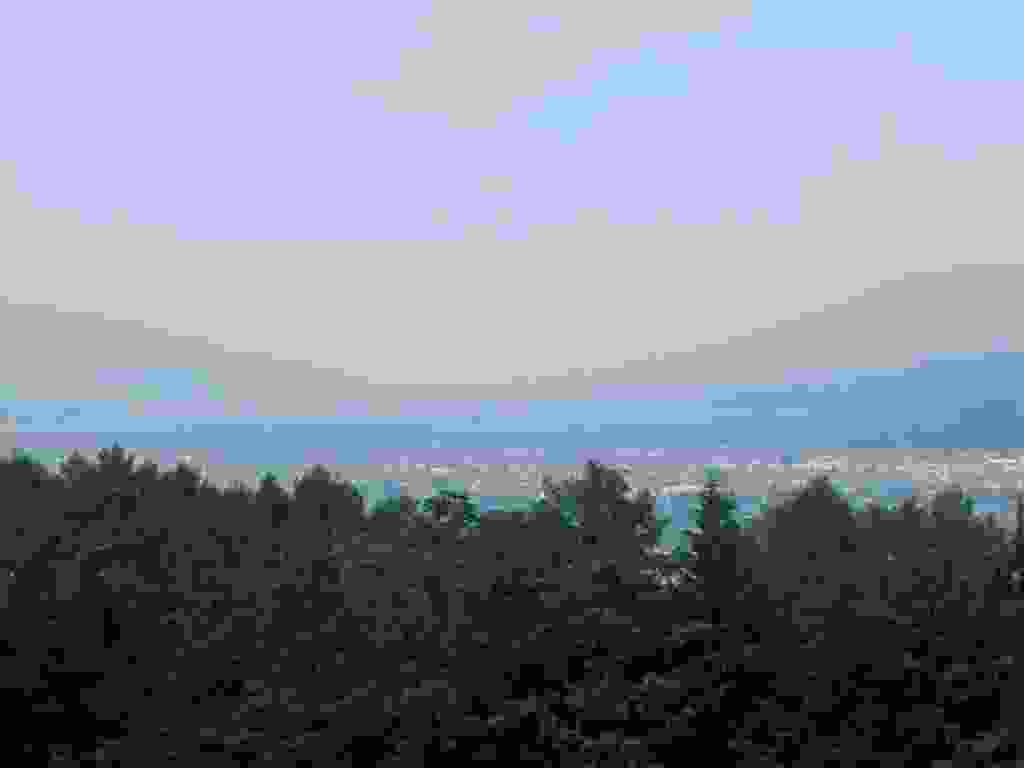
\includegraphics[width=\mywidth]{../wp-content/uploads/2015/08/P8035933-1024x768.jpg} \end{center}

 

 A la sortie de la ville, je m'arrête dans un magasin de vélo pour changer les plateaux et la chaine. Le technicien monte la chaine neuve que j'avais déjà et 2 plateaux récupérés sur un vélo dans le magasin. A la fin je demande pour payer mais il me dit simplement «Good bye it's service», incroyable ! 

 

\begin{center} 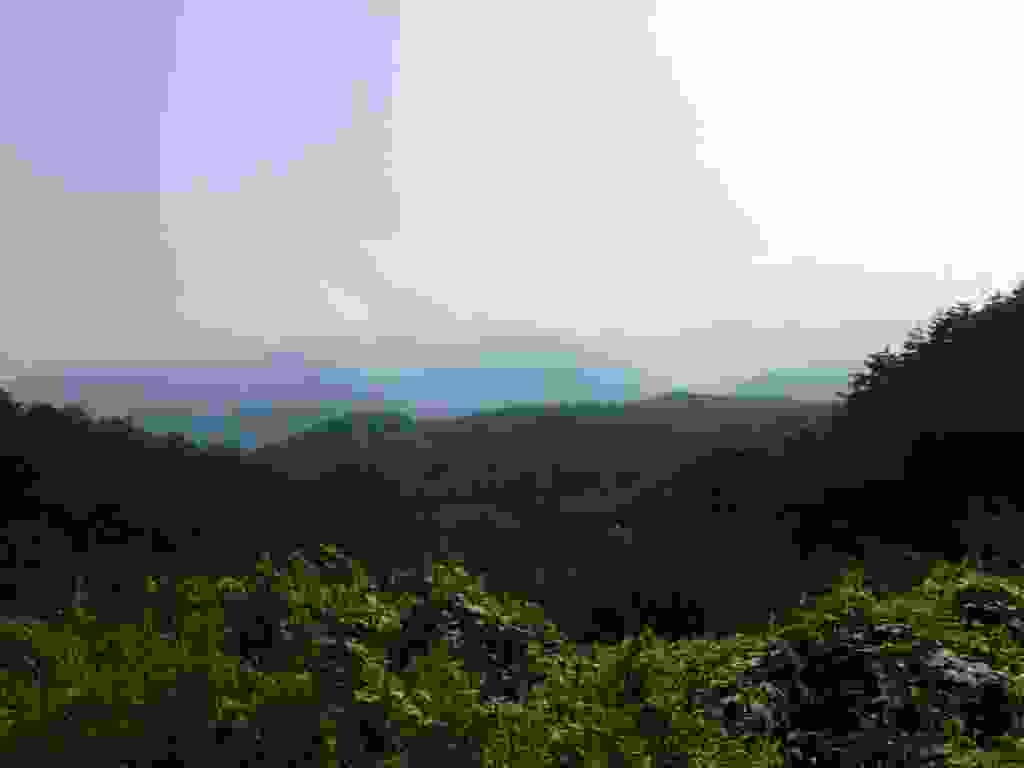
\includegraphics[width=\mywidth]{../wp-content/uploads/2015/08/P8045944-1024x768.jpg} \end{center}

 

 A Matsumoto, visite du célèbre chateau qui est d'origine, contrairement à beaucoup de chateaux au Japon. 

 

\begin{center} 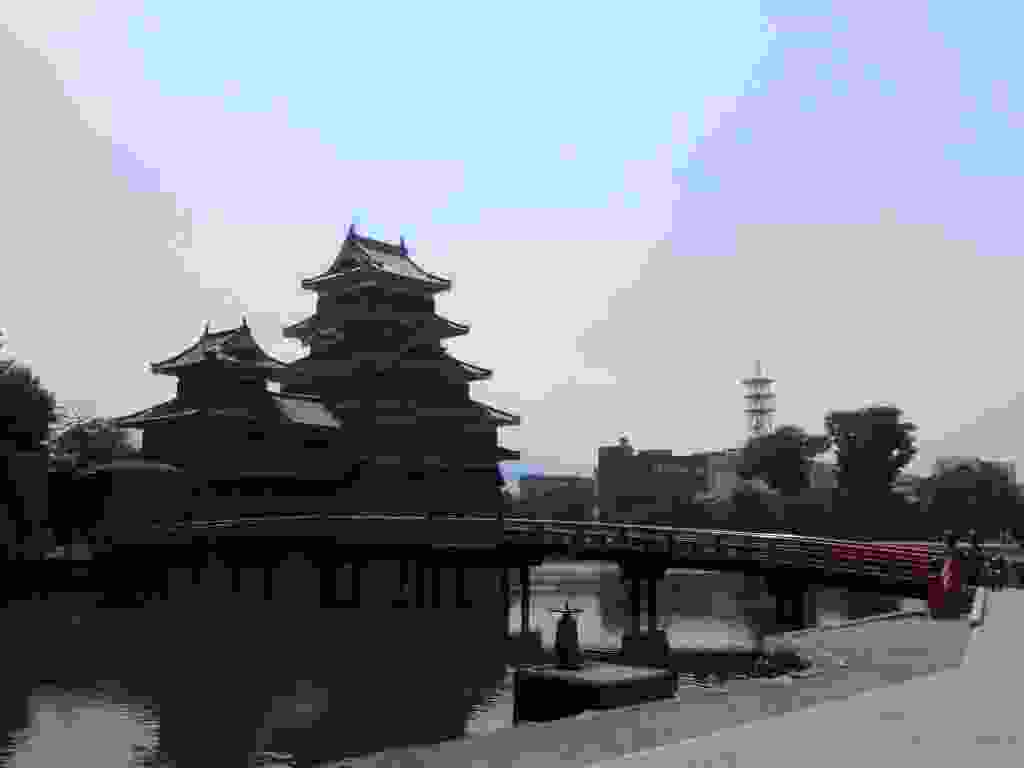
\includegraphics[width=\mywidth]{../wp-content/uploads/2015/08/P8045947-1024x768.jpg} \end{center}

 

 

\begin{center} 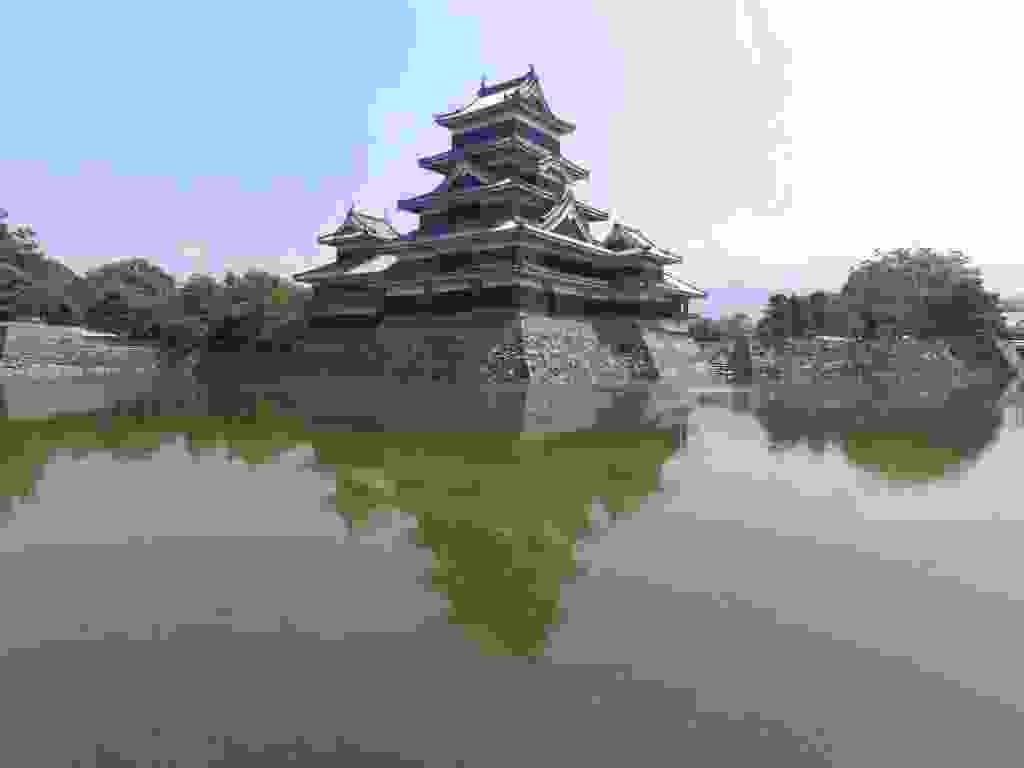
\includegraphics[width=\mywidth]{../wp-content/uploads/2015/08/P8045951-1024x768.jpg} \end{center}

 

 

\begin{center} 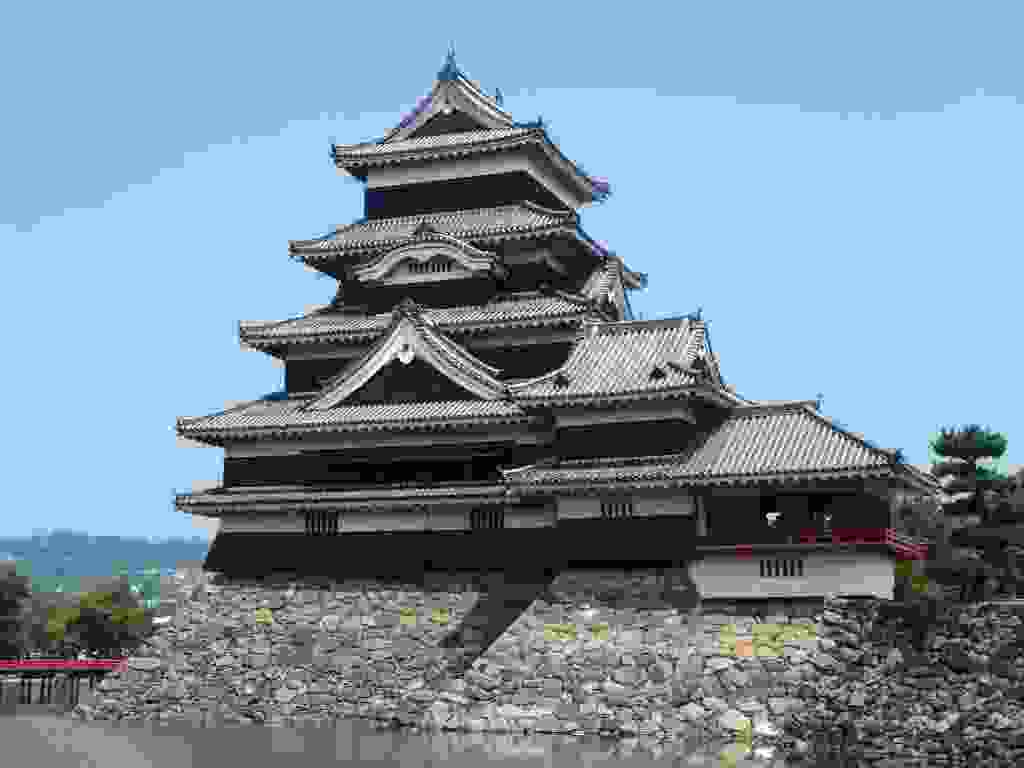
\includegraphics[width=\mywidth]{../wp-content/uploads/2015/08/P8045953-1024x768.jpg} \end{center}

 

 

\begin{center} 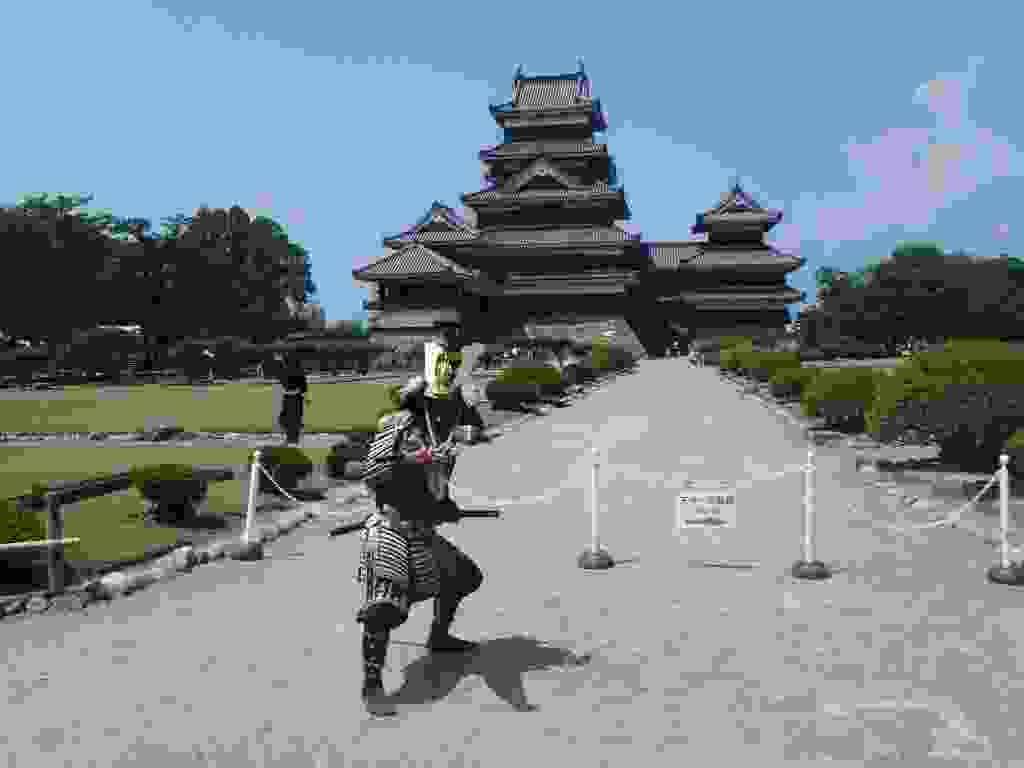
\includegraphics[width=\mywidth]{../wp-content/uploads/2015/08/P8045959-1024x768.jpg} \end{center}

 

 

\begin{center} 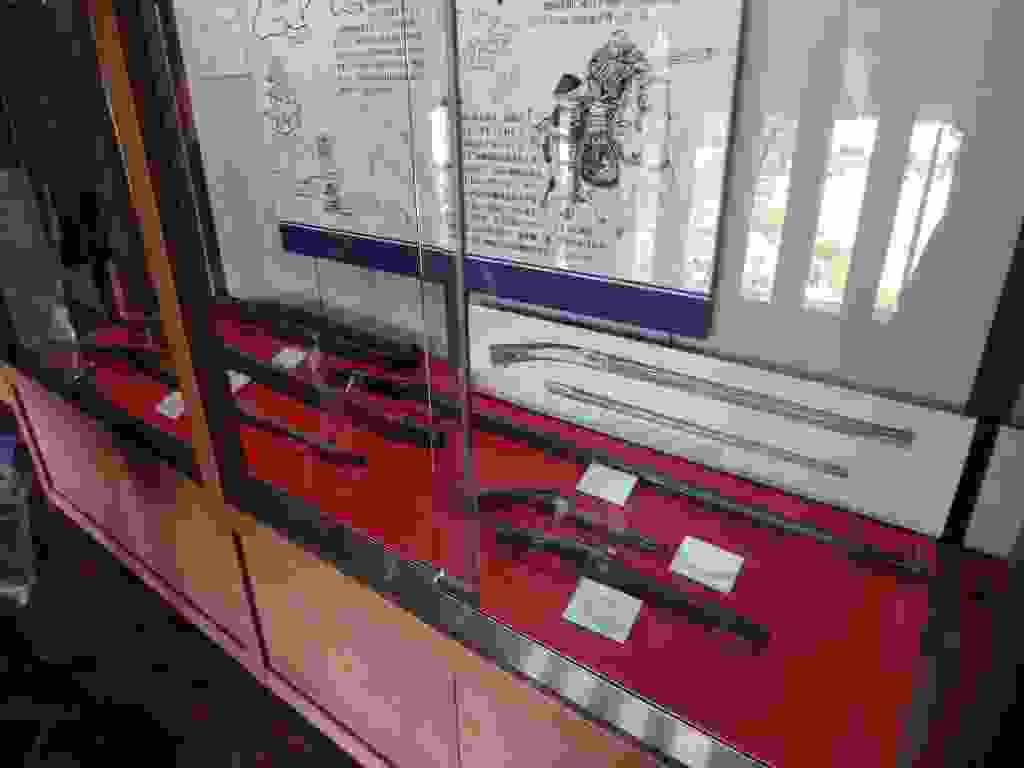
\includegraphics[width=\mywidth]{../wp-content/uploads/2015/08/P8045961-1024x768.jpg} \end{center}

 

 Ensuite la route monte pour entrer dans les Alpes Japonaises, portion pas toujours agréable avec beaucoup de tunnels dont un de 2km en montée à plus de 12%. 

 

\begin{center} 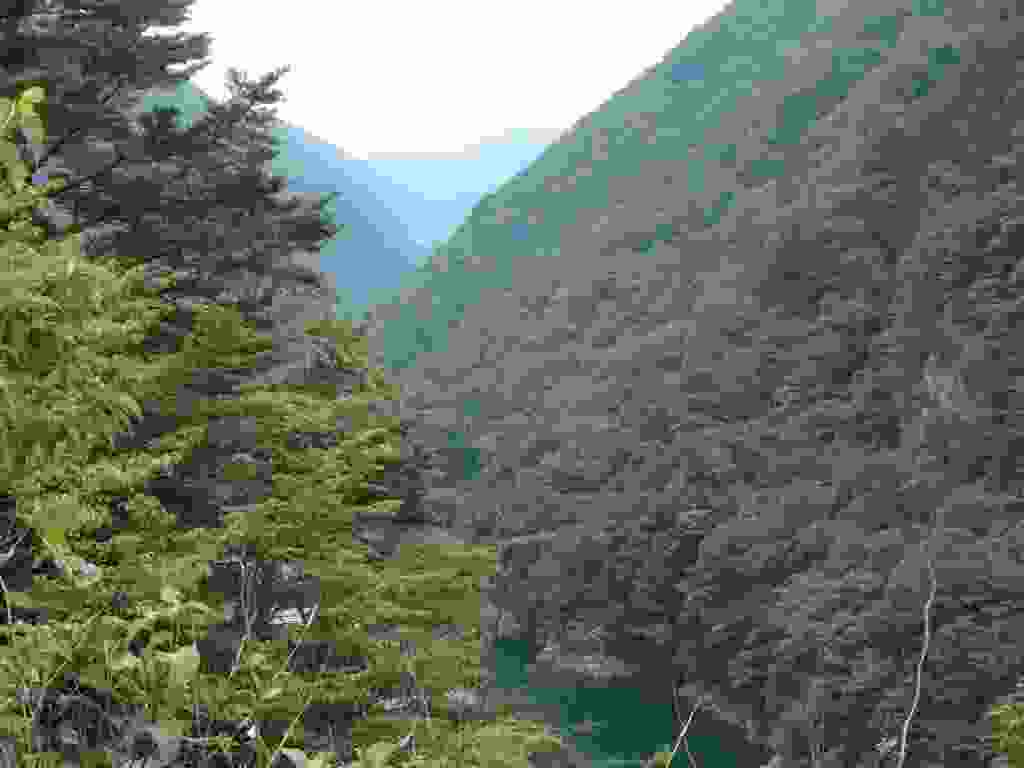
\includegraphics[width=\mywidth]{../wp-content/uploads/2015/08/P8045969-1024x768.jpg} \end{center}

 

 

\begin{center} 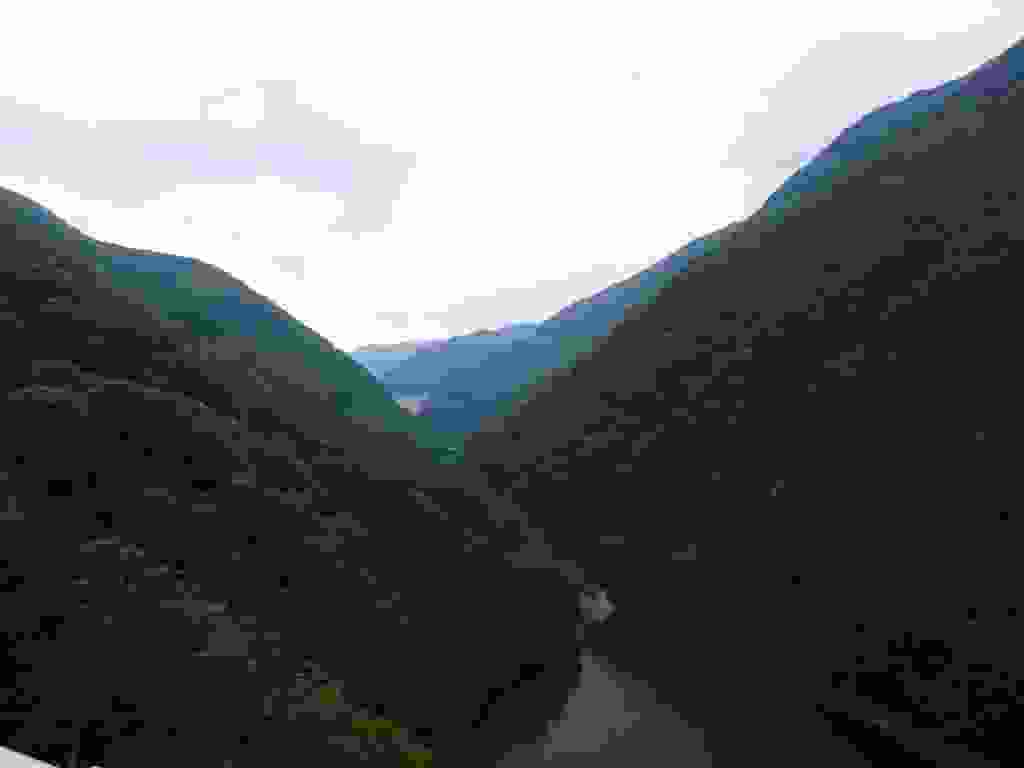
\includegraphics[width=\mywidth]{../wp-content/uploads/2015/08/P8045970-1024x768.jpg} \end{center}

 

 

\begin{center} 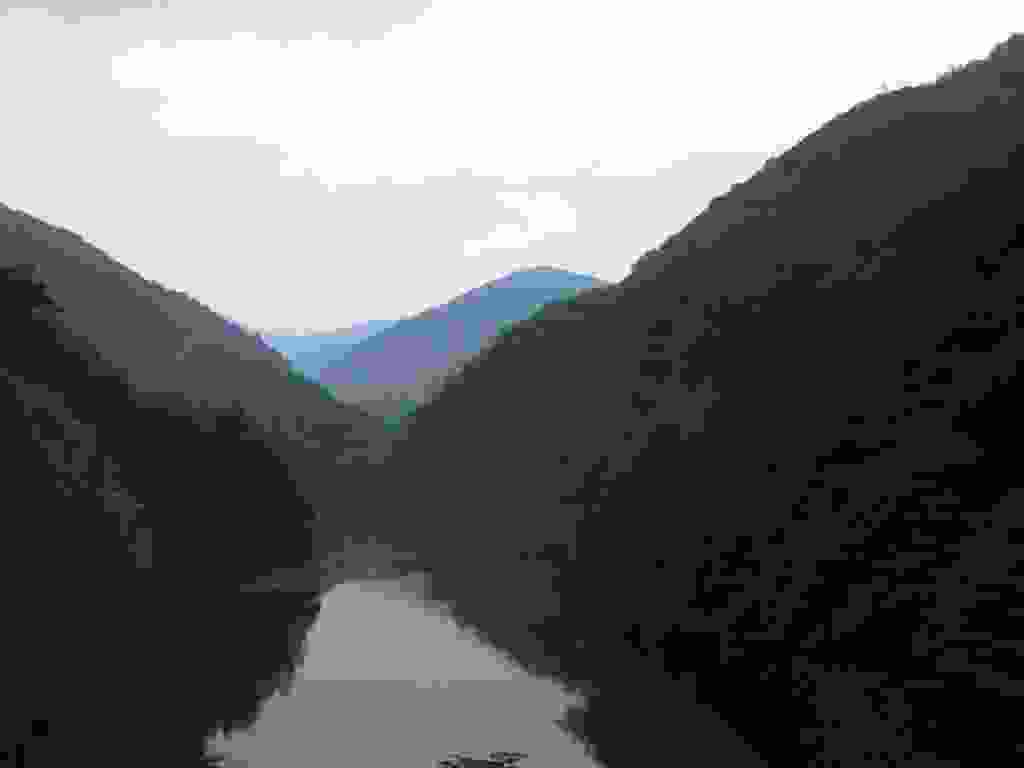
\includegraphics[width=\mywidth]{../wp-content/uploads/2015/08/P8045972-1024x768.jpg} \end{center}

 

 La montée se termine à Kamikochi par une portion de route plus tranquille ouverte seulement aux bus et aux taxis. 

 

\begin{center} 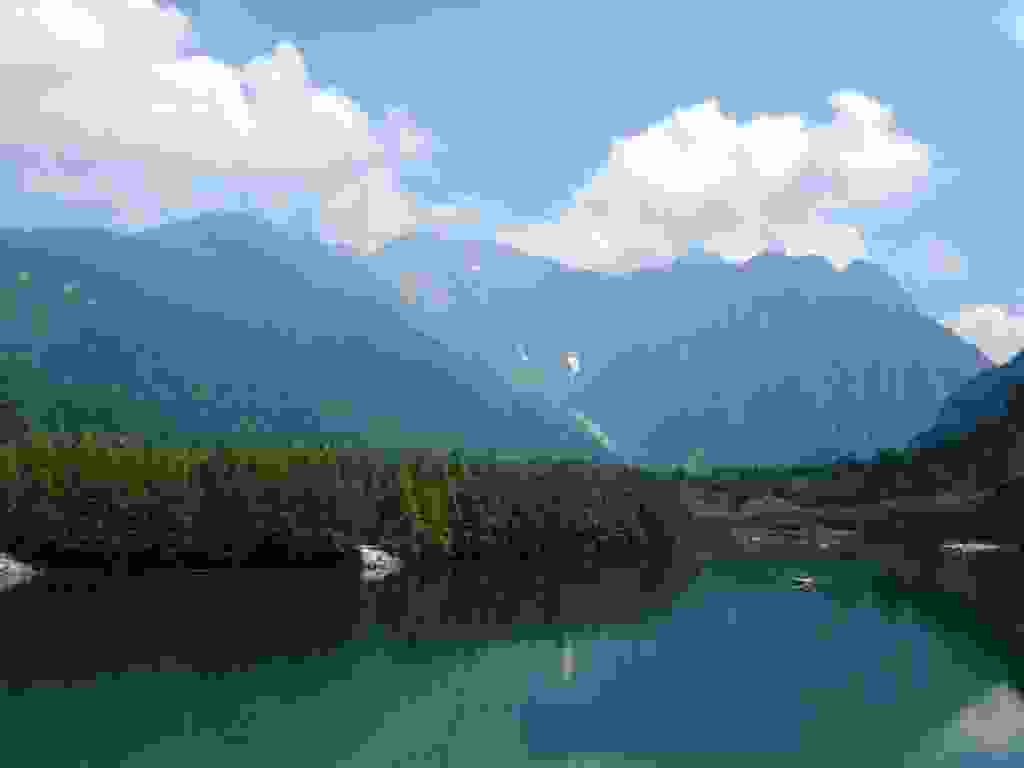
\includegraphics[width=\mywidth]{../wp-content/uploads/2015/08/P8055978-1024x768.jpg} \end{center}

 

 

\begin{center} 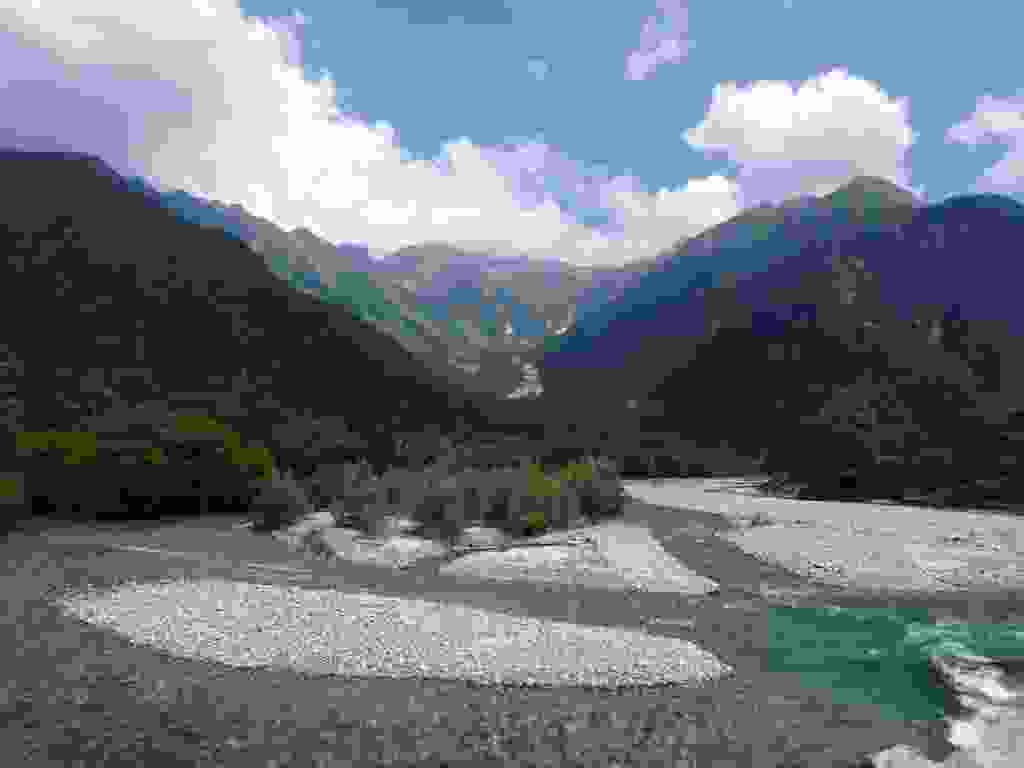
\includegraphics[width=\mywidth]{../wp-content/uploads/2015/08/P8055985-1024x768.jpg} \end{center}

 

 C'est le lieu de départ de plusieurs randonnées et ascensions, j'en profite pour monter jusqu'à un refuge à 2200m. 

 

\begin{center} 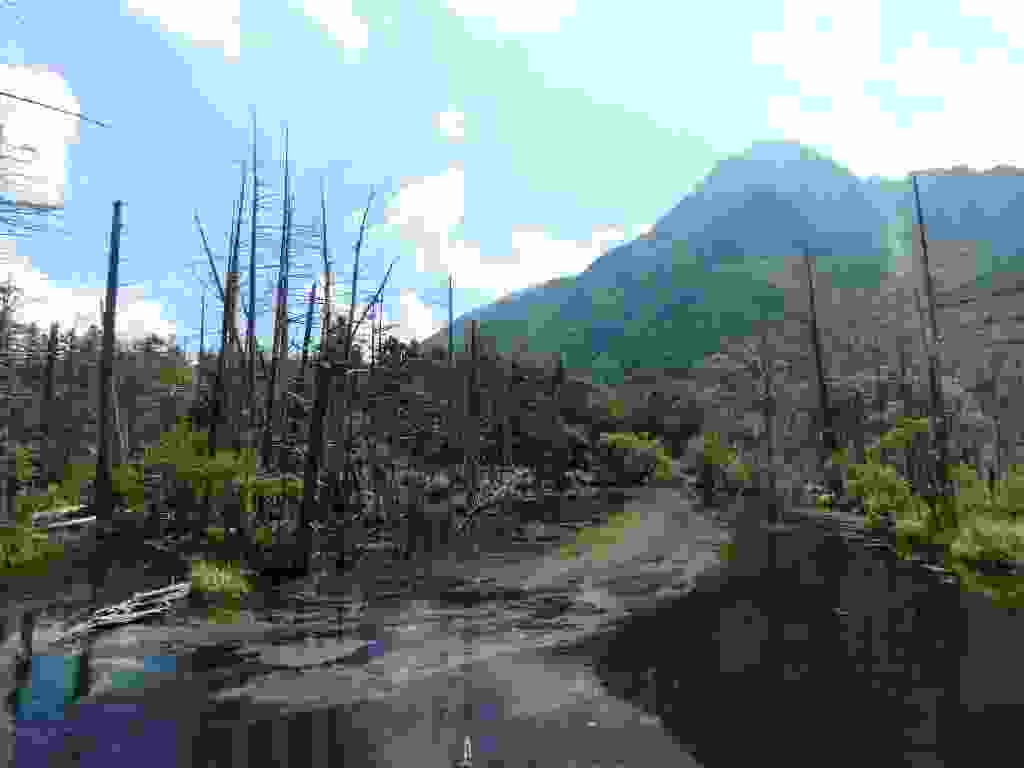
\includegraphics[width=\mywidth]{../wp-content/uploads/2015/08/P8055987-1024x768.jpg} \end{center}

 

 

\begin{center} 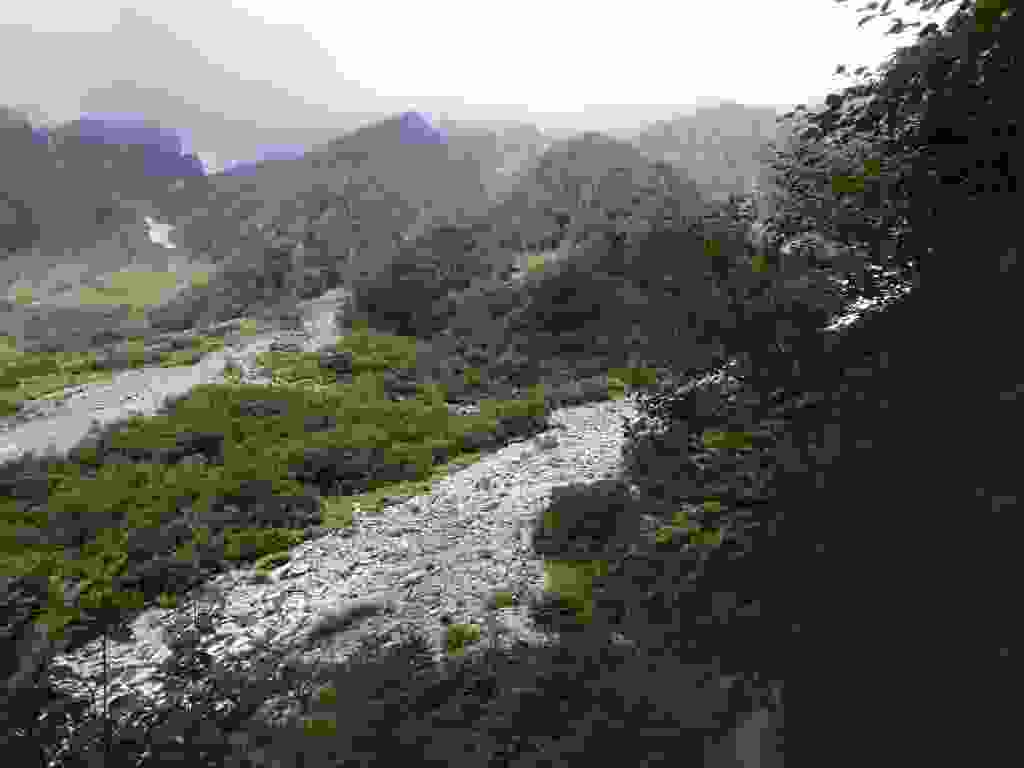
\includegraphics[width=\mywidth]{../wp-content/uploads/2015/08/P8055990-1024x768.jpg} \end{center}

 

 

\begin{center} 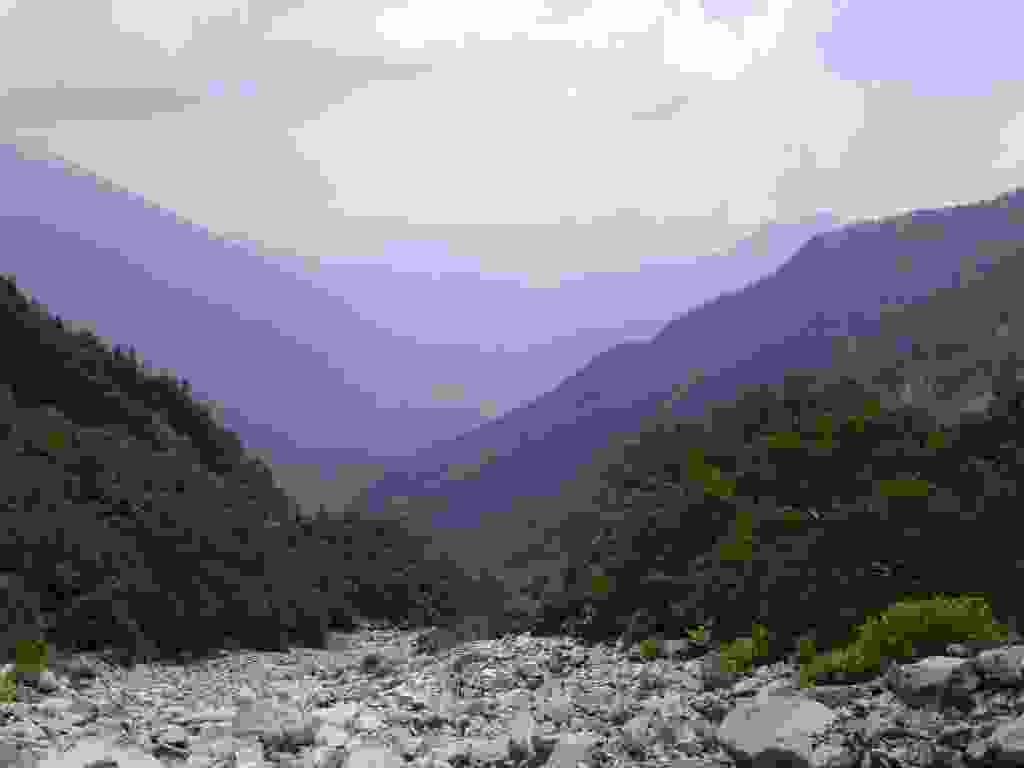
\includegraphics[width=\mywidth]{../wp-content/uploads/2015/08/P8055993-1024x768.jpg} \end{center}

 

 

\begin{center} 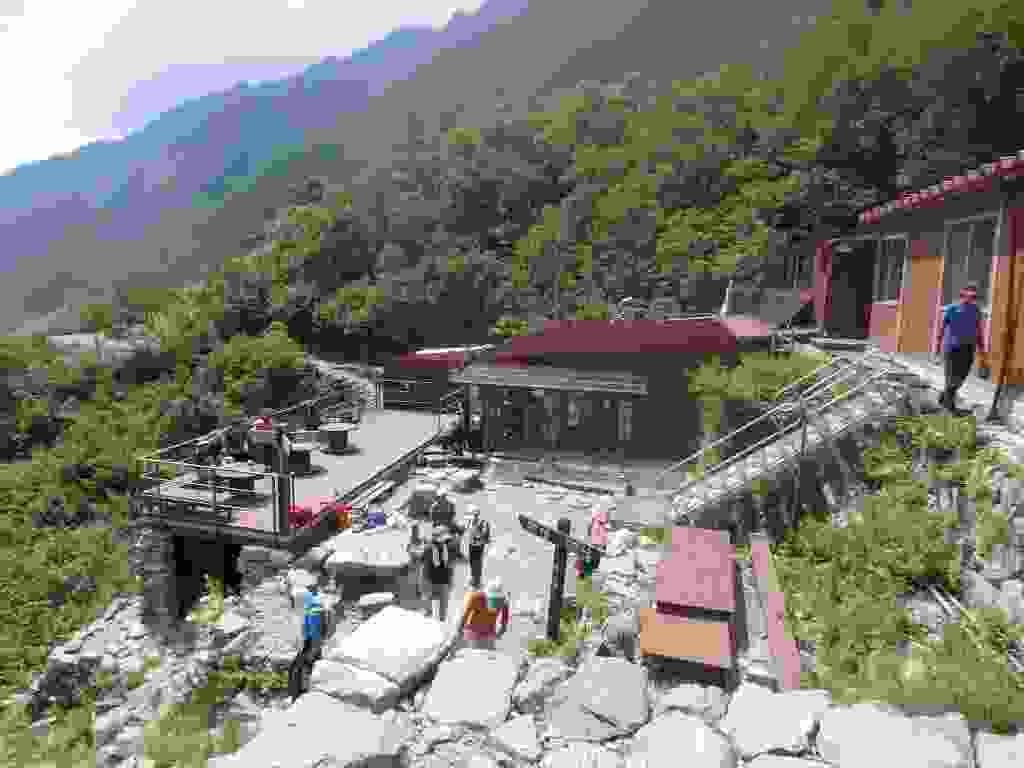
\includegraphics[width=\mywidth]{../wp-content/uploads/2015/08/P8055998-1024x768.jpg} \end{center}

 

 En fin d'après midi je redescends un peu et me lance dans un nouveau col quand je suis surpris par un orage. La pluie ne s'arrête pas, je me decide à poser la tente : idée moyenne, tout est trempé y compris l'intérieur qui est une grosse flaque ! 

 

\begin{center} 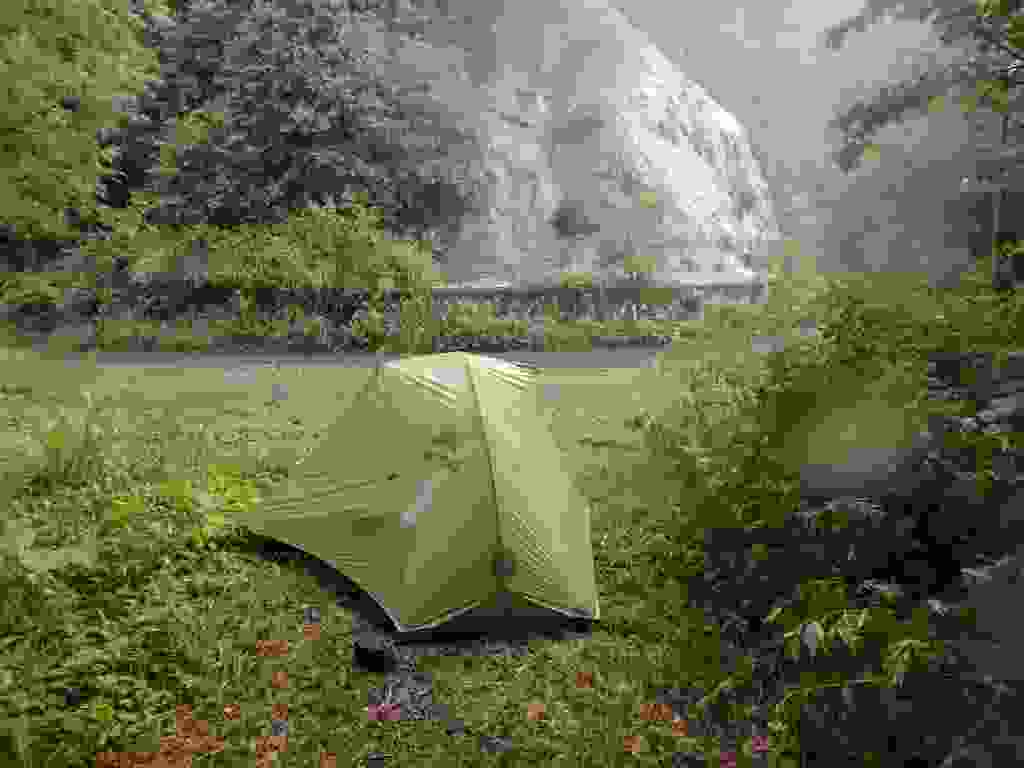
\includegraphics[width=\mywidth]{../wp-content/uploads/2015/08/P8056003-1024x768.jpg} \end{center}

 

 

\begin{center} 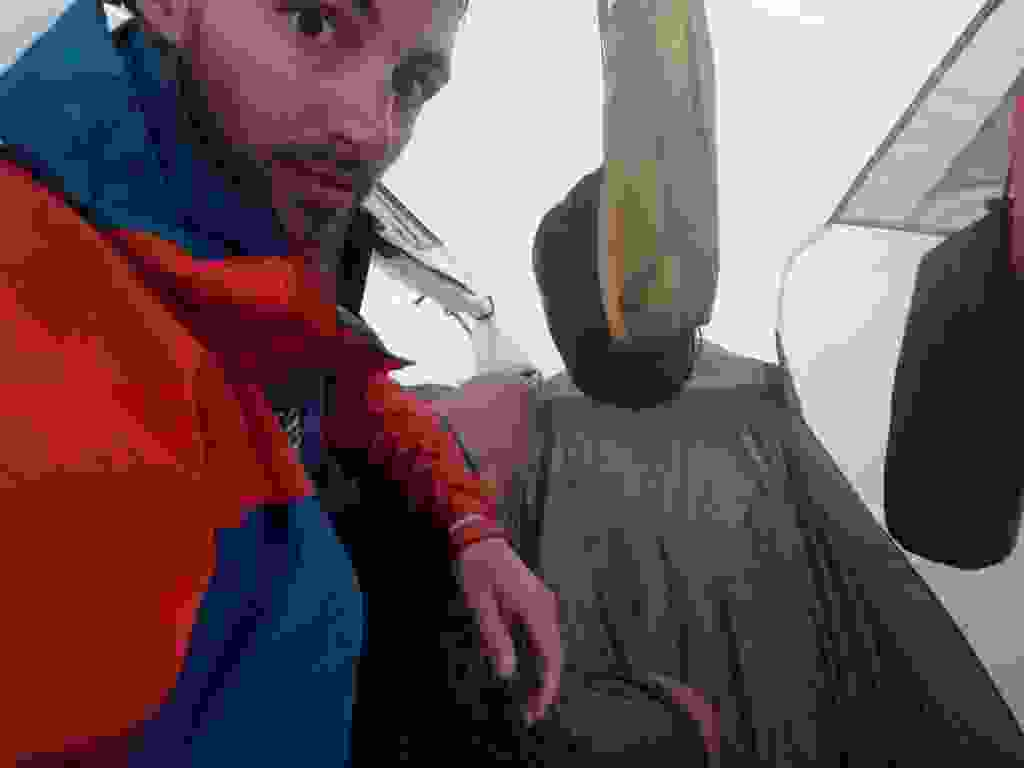
\includegraphics[width=\mywidth]{../wp-content/uploads/2015/08/P8056001-1024x768.jpg} \end{center}

 

 Après 2 autres cols, une longue descente me mène à Takayama ou je reste 2 jours dans un hotel pour me reposer et sécher complètement. 

 

\begin{center} 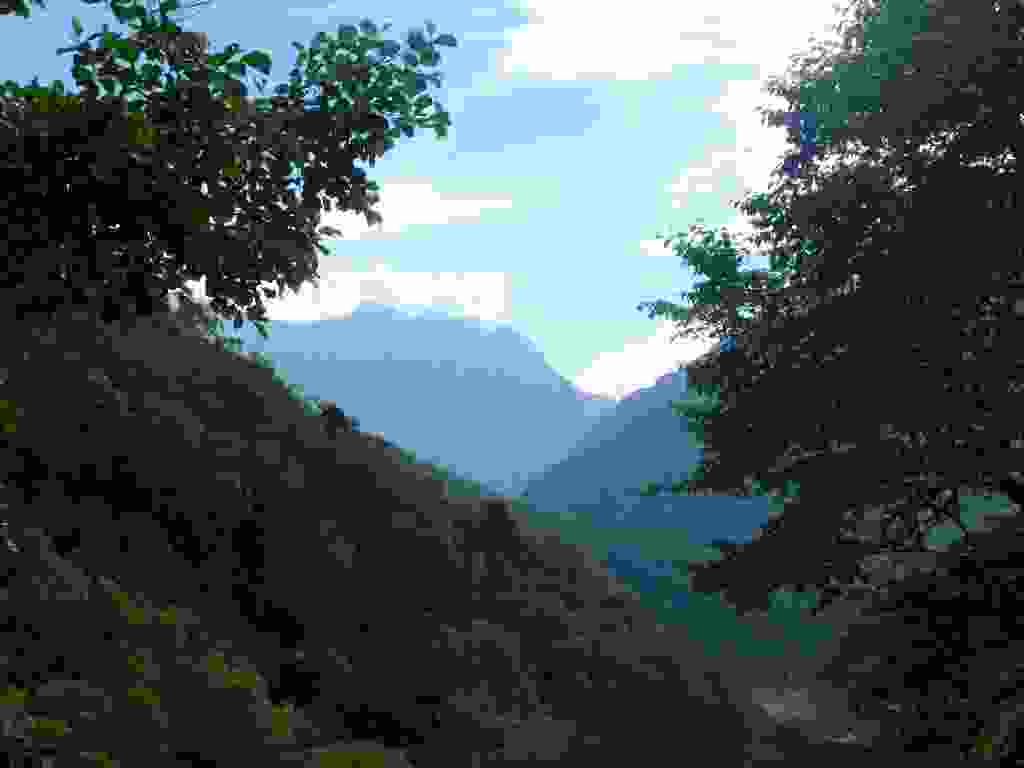
\includegraphics[width=\mywidth]{../wp-content/uploads/2015/08/P8066004-1024x768.jpg} \end{center}

 

 

\begin{center} 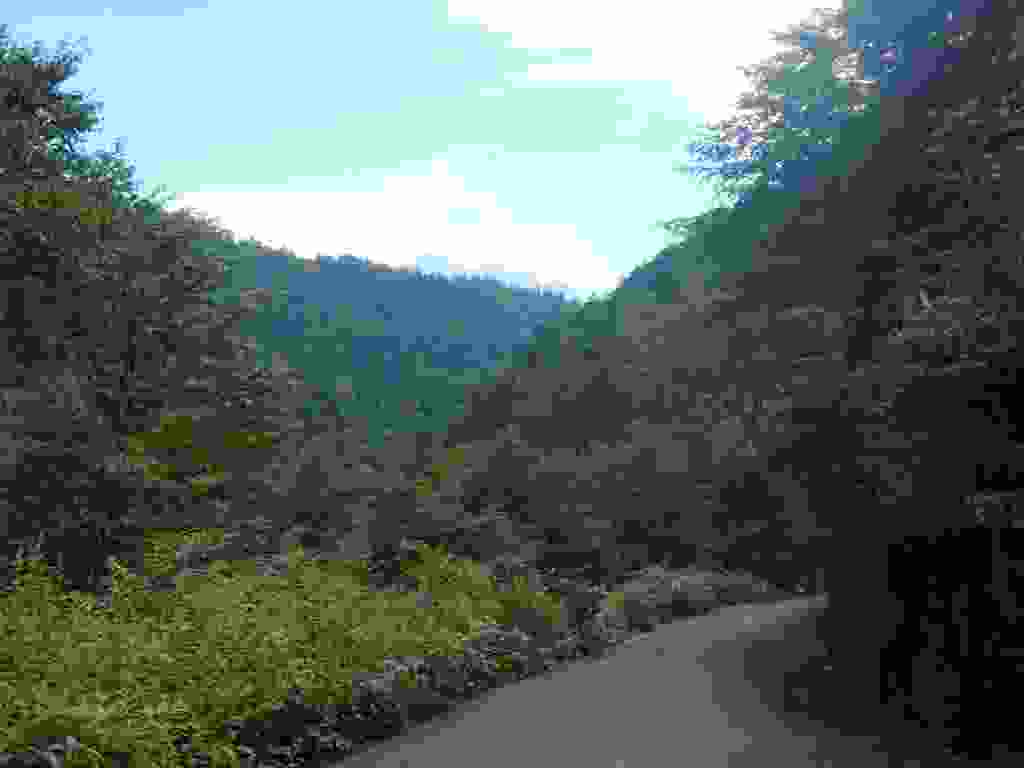
\includegraphics[width=\mywidth]{../wp-content/uploads/2015/08/P8066005-1024x768.jpg} \end{center}

 

 

\begin{center} 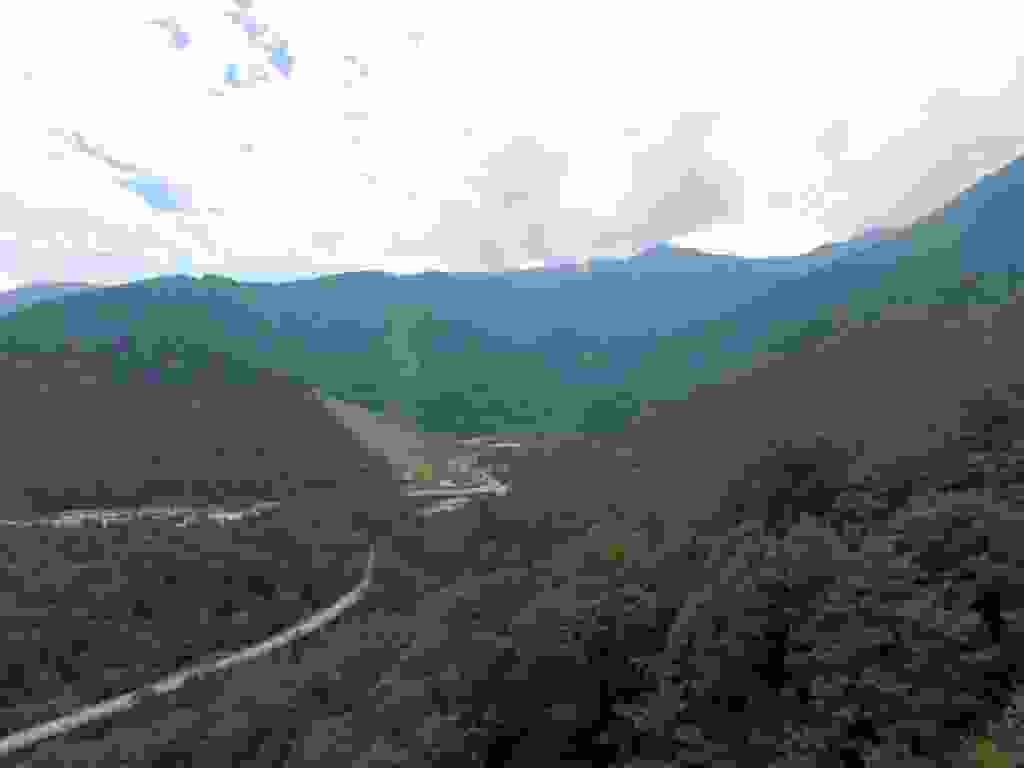
\includegraphics[width=\mywidth]{../wp-content/uploads/2015/08/P8066012-1024x768.jpg} \end{center}

 

 Un petit marché se tient au bord de la rivière. 

 

\begin{center} 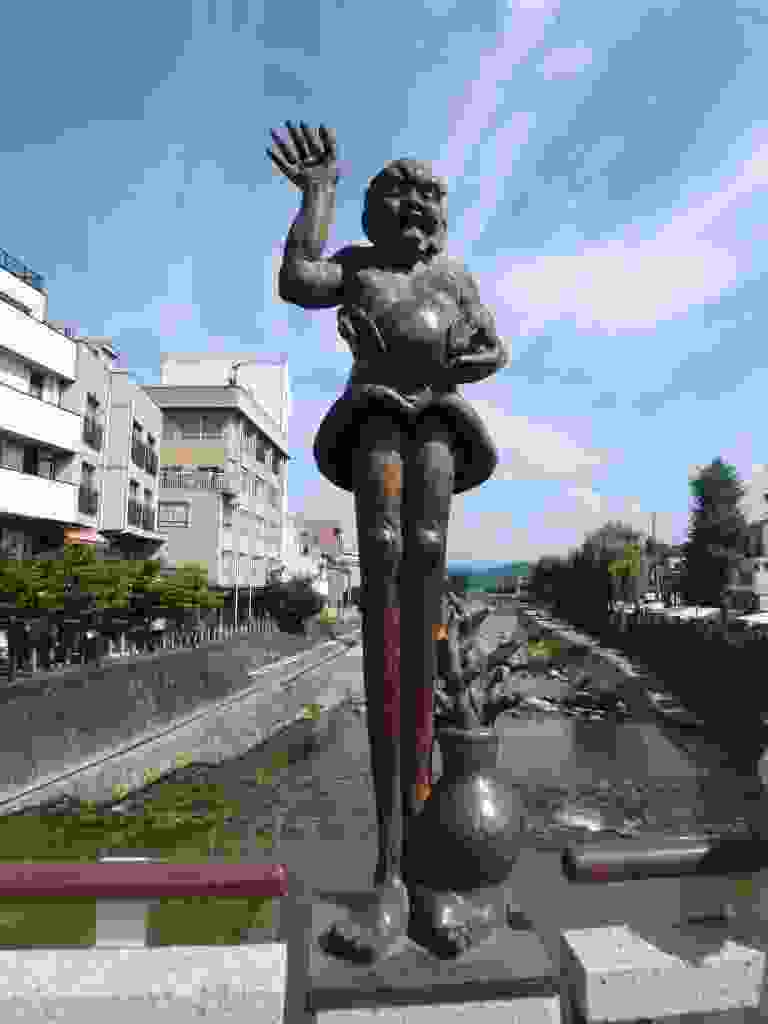
\includegraphics[width=\mywidth]{../wp-content/uploads/2015/08/P8076023-e1439361015244-768x1024.jpg} \end{center}

 

 

\begin{center} 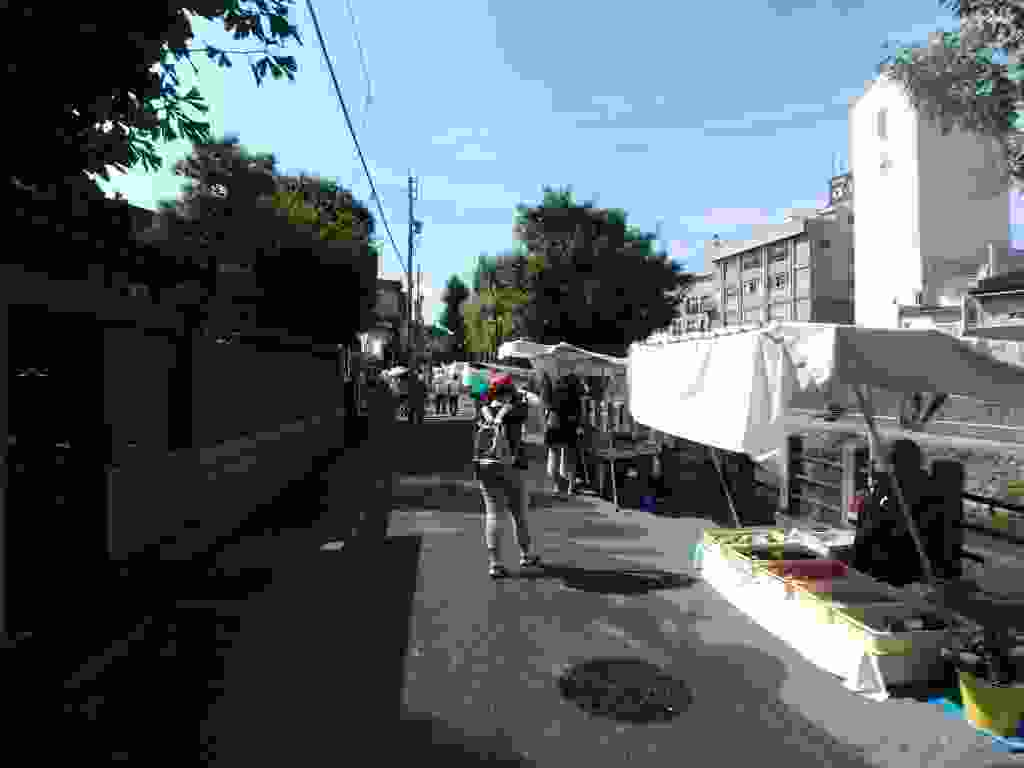
\includegraphics[width=\mywidth]{../wp-content/uploads/2015/08/P8076021-1024x768.jpg} \end{center}

 

 Beaucoup de maisons traditionnelles en bois dans le centre ville. 

 

\begin{center} 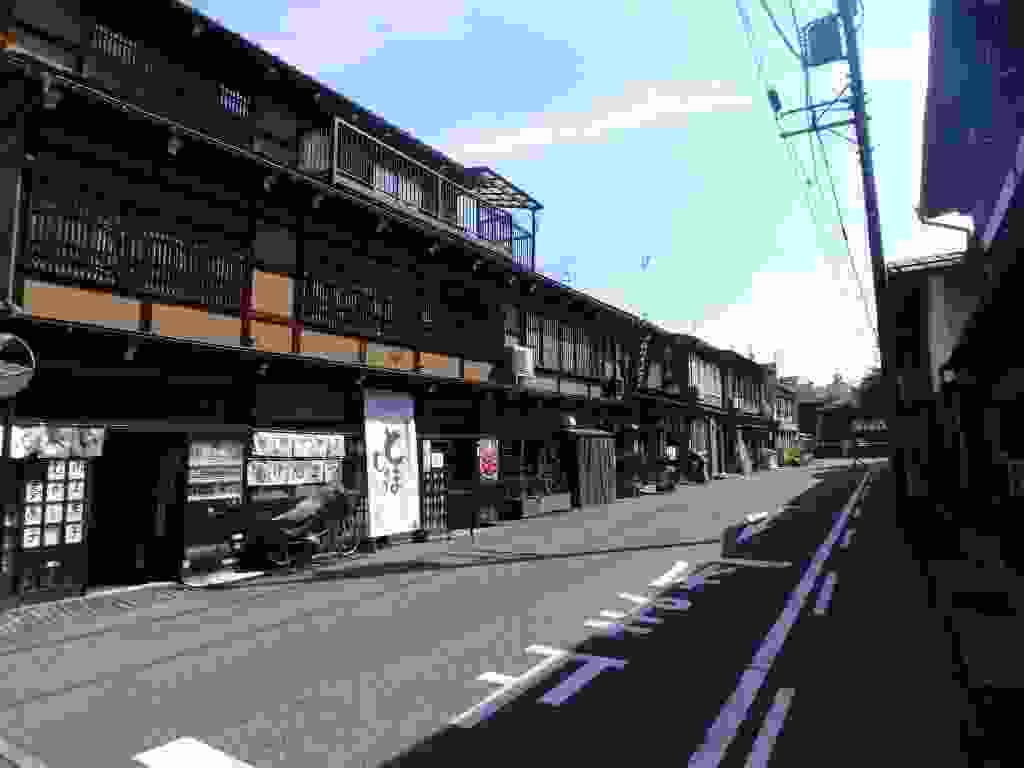
\includegraphics[width=\mywidth]{../wp-content/uploads/2015/08/P8076026-1024x768.jpg} \end{center}

 

 

\begin{center} 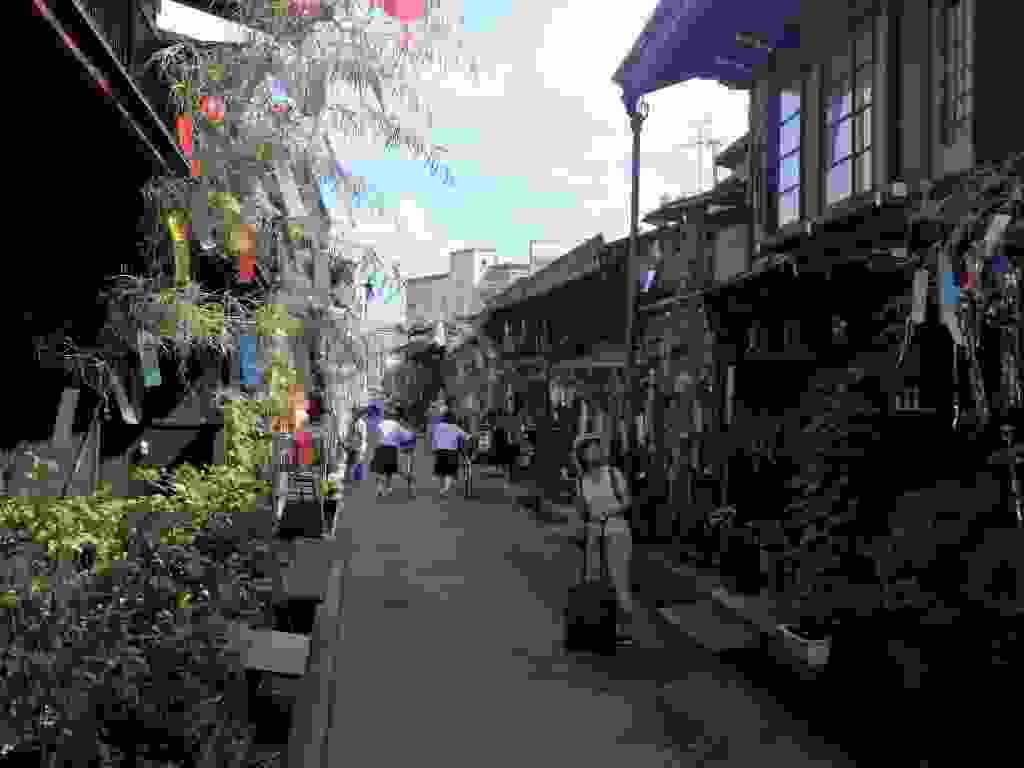
\includegraphics[width=\mywidth]{../wp-content/uploads/2015/08/P8076030-1024x768.jpg} \end{center}

 

 

\begin{center} 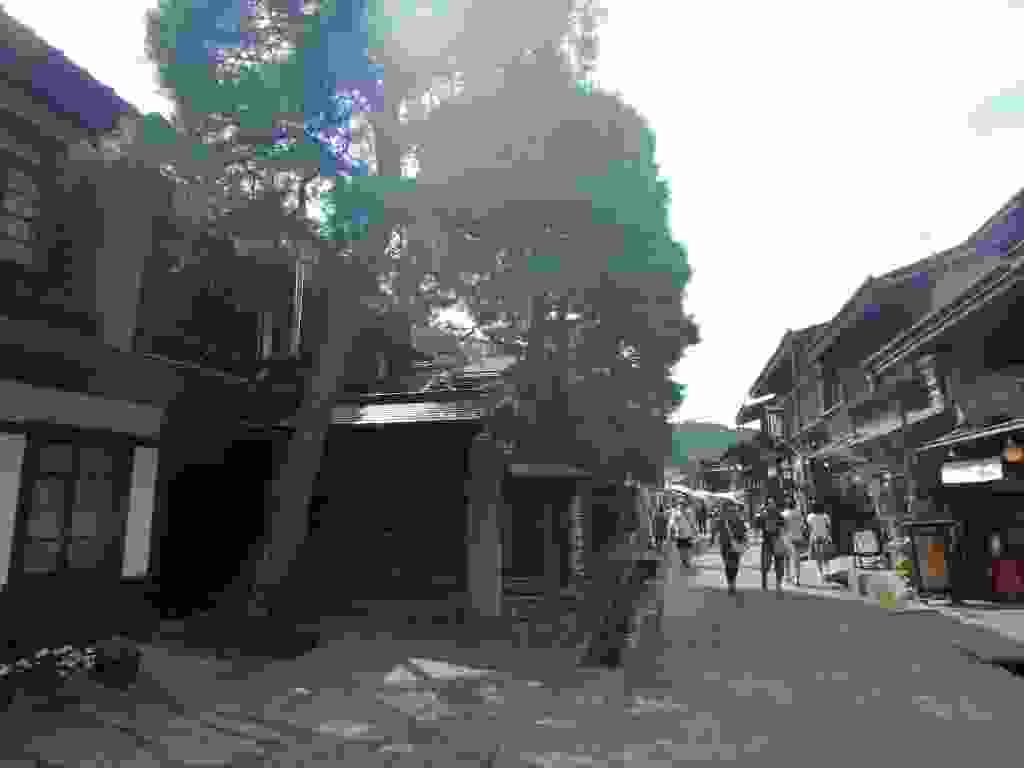
\includegraphics[width=\mywidth]{../wp-content/uploads/2015/08/P8076034-1024x768.jpg} \end{center}

 

 

\begin{center} 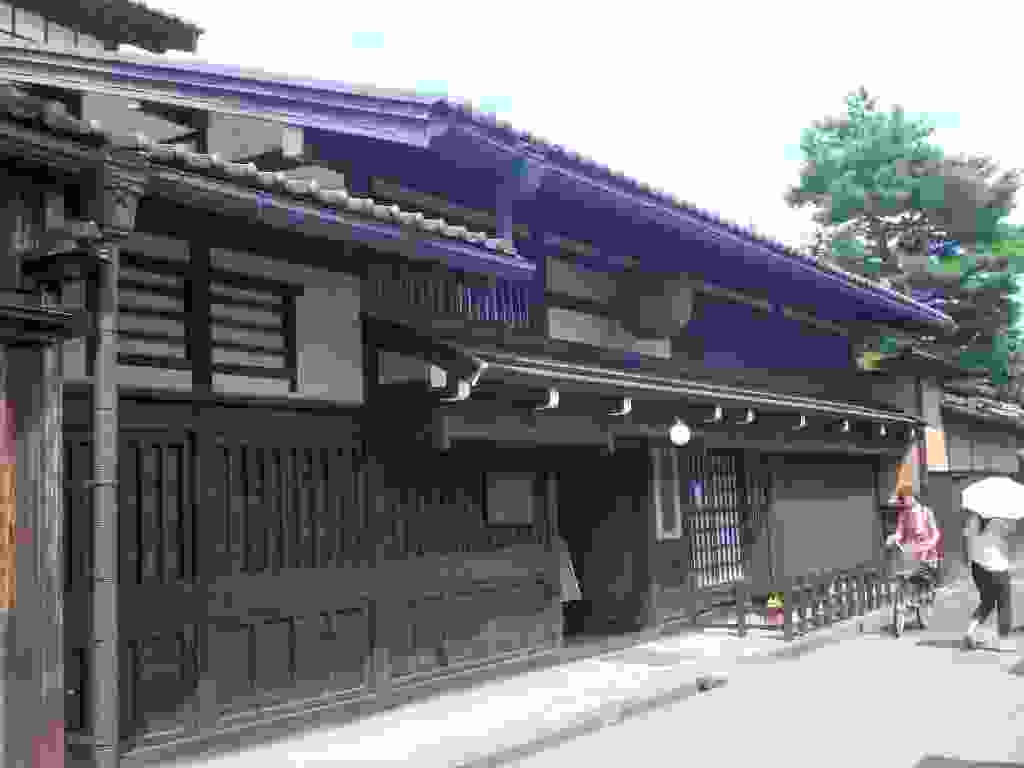
\includegraphics[width=\mywidth]{../wp-content/uploads/2015/08/P8076041-1024x768.jpg} \end{center}

 

 Boutique spécialisée dans le saké. 

 

\begin{center} 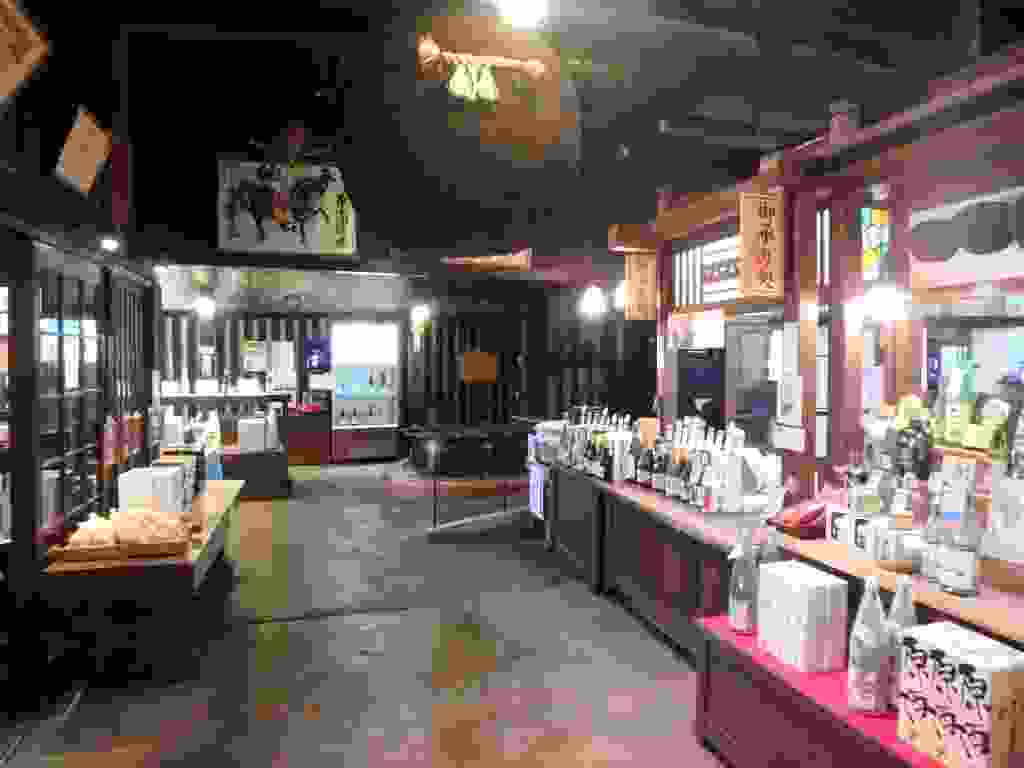
\includegraphics[width=\mywidth]{../wp-content/uploads/2015/08/P8076032-1024x768.jpg} \end{center}

 

 Un quartier avec une dizaine de temples les uns à coté des autres. 

 

\begin{center} 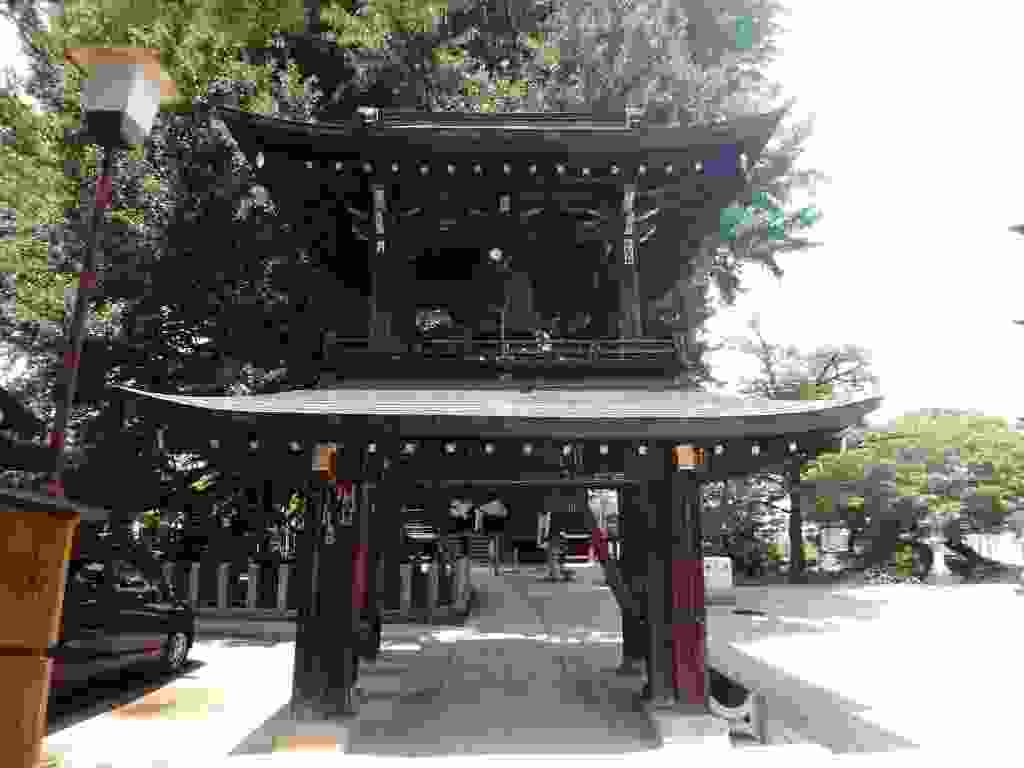
\includegraphics[width=\mywidth]{../wp-content/uploads/2015/08/P8066014-1024x768.jpg} \end{center}

 

 

\begin{center} 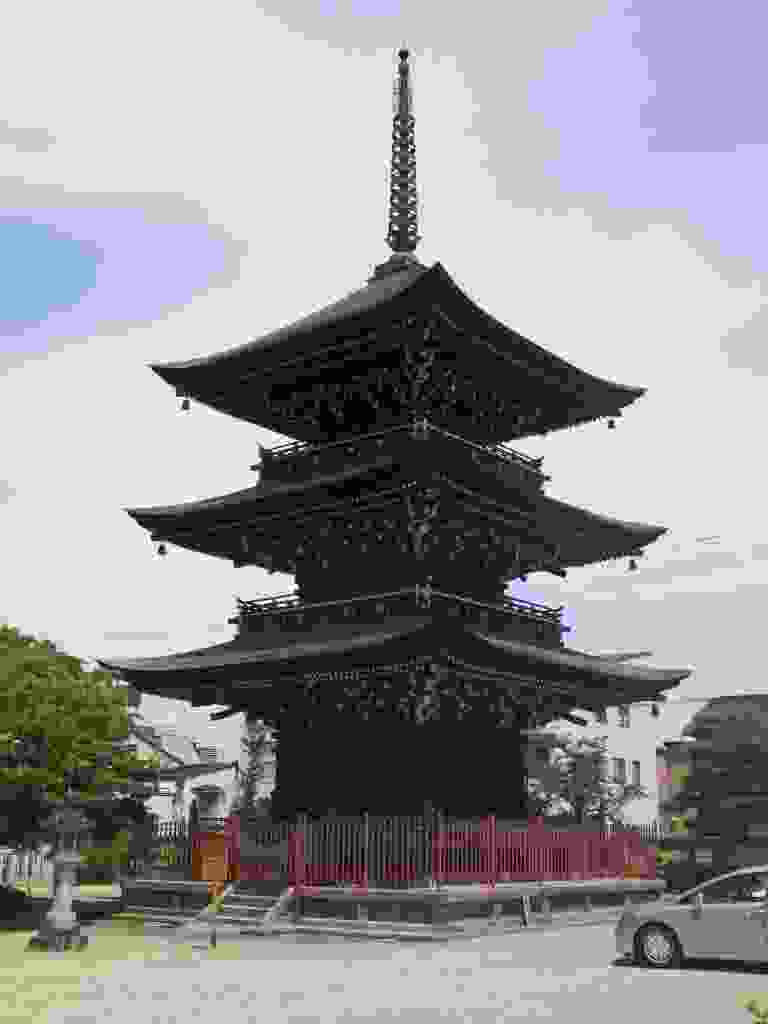
\includegraphics[width=\mywidth]{../wp-content/uploads/2015/08/P8066015-e1439361164467-768x1024.jpg} \end{center}

 

 

\begin{center} 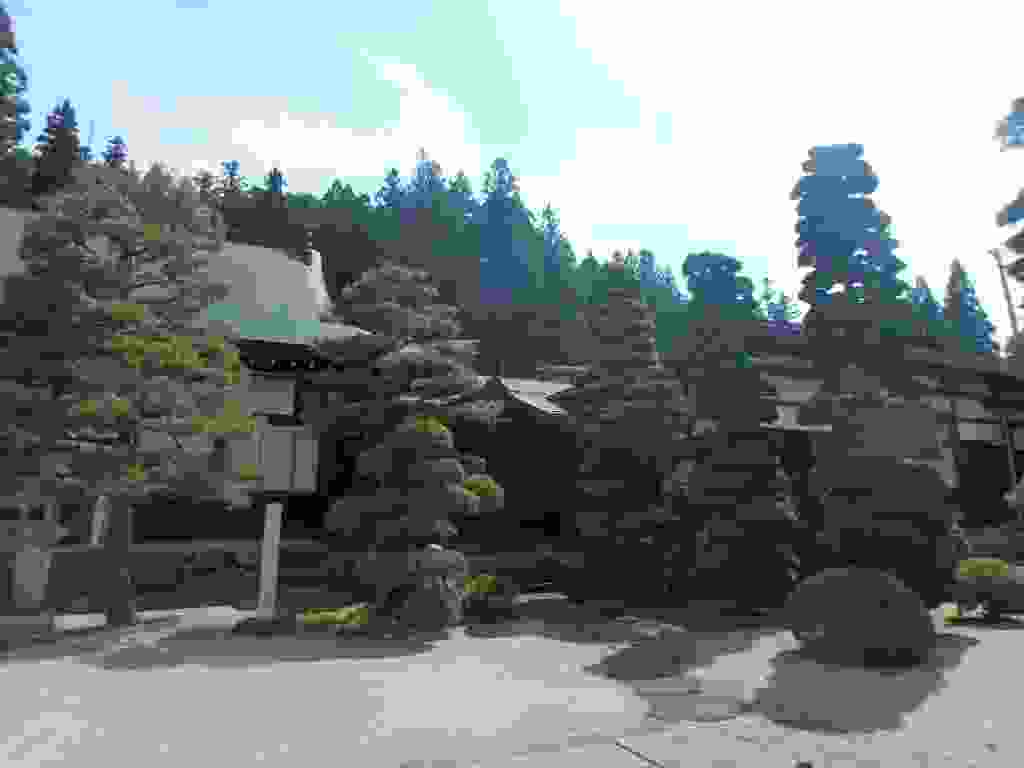
\includegraphics[width=\mywidth]{../wp-content/uploads/2015/08/P8076042-1024x768.jpg} \end{center}

 

 

\begin{center} 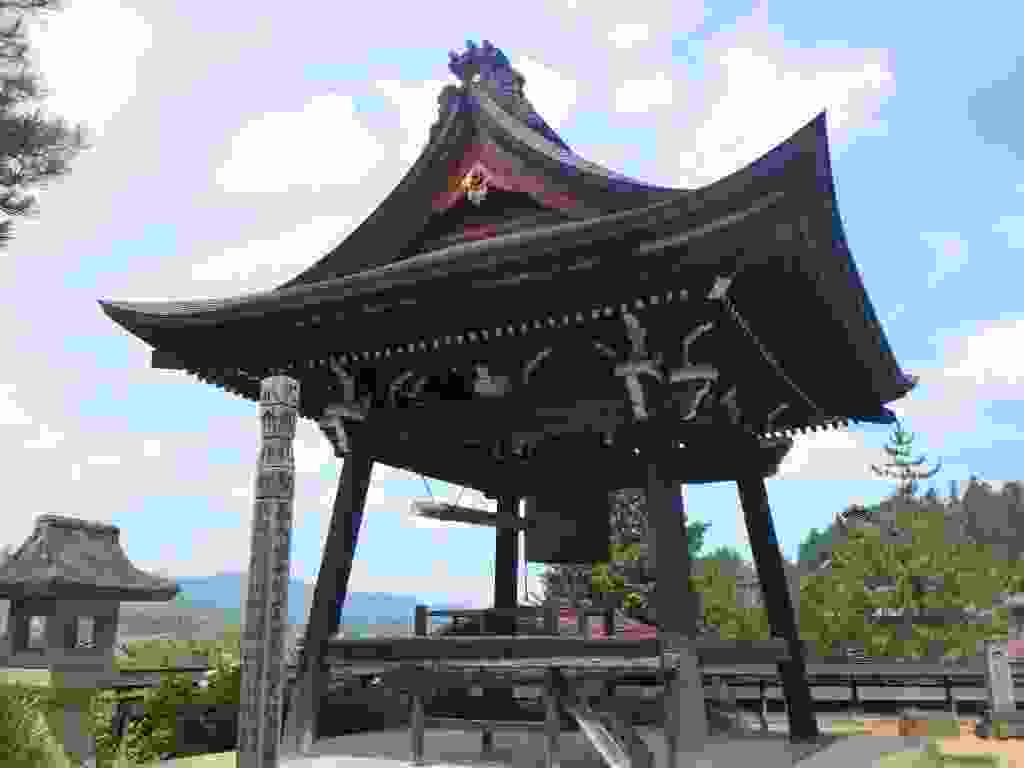
\includegraphics[width=\mywidth]{../wp-content/uploads/2015/08/P8076053-1024x768.jpg} \end{center}

 

 

\begin{center} 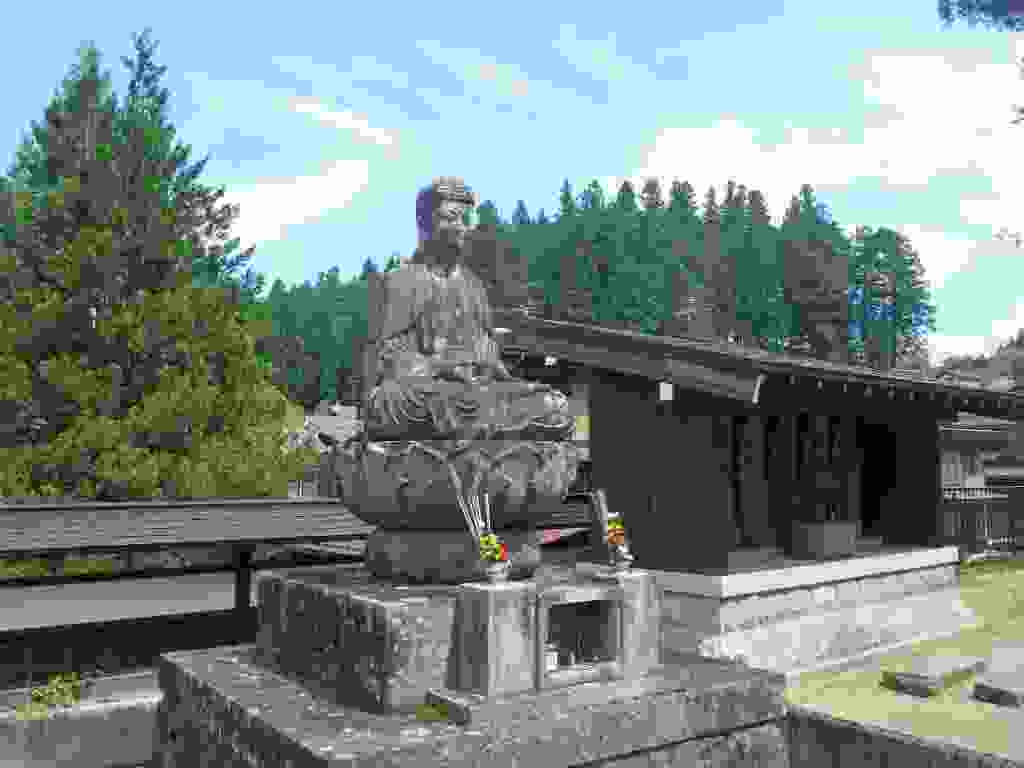
\includegraphics[width=\mywidth]{../wp-content/uploads/2015/08/P8076054-1024x768.jpg} \end{center}

 

 

\begin{center} 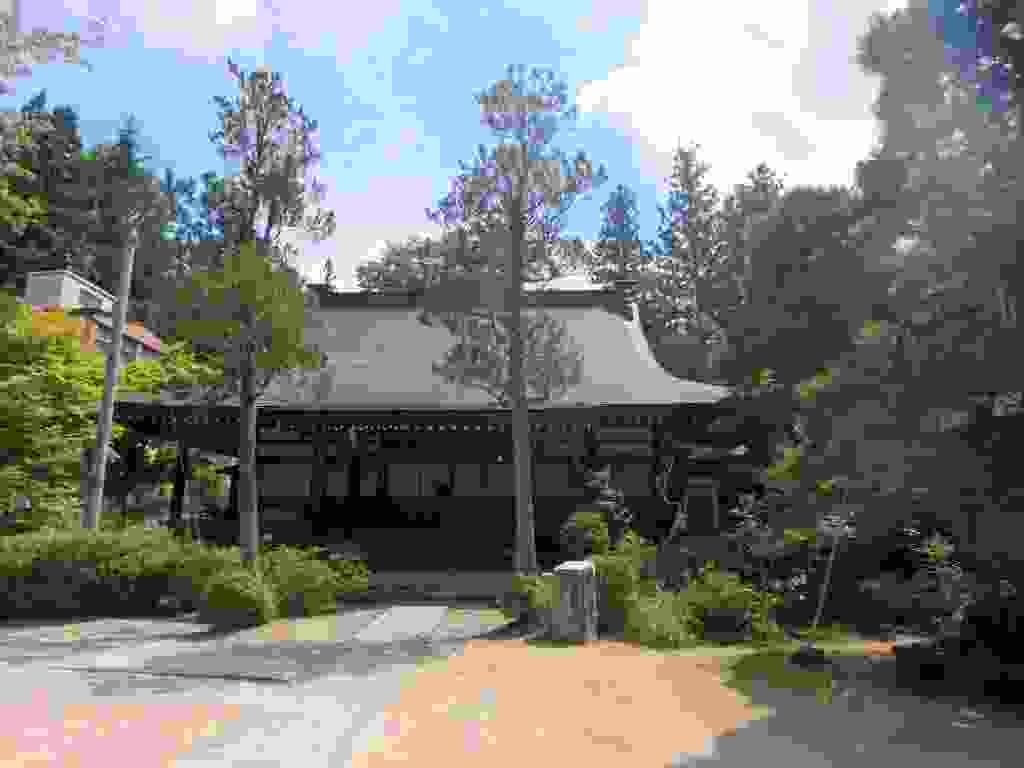
\includegraphics[width=\mywidth]{../wp-content/uploads/2015/08/P8076057-1024x768.jpg} \end{center}

 

 

\begin{center} 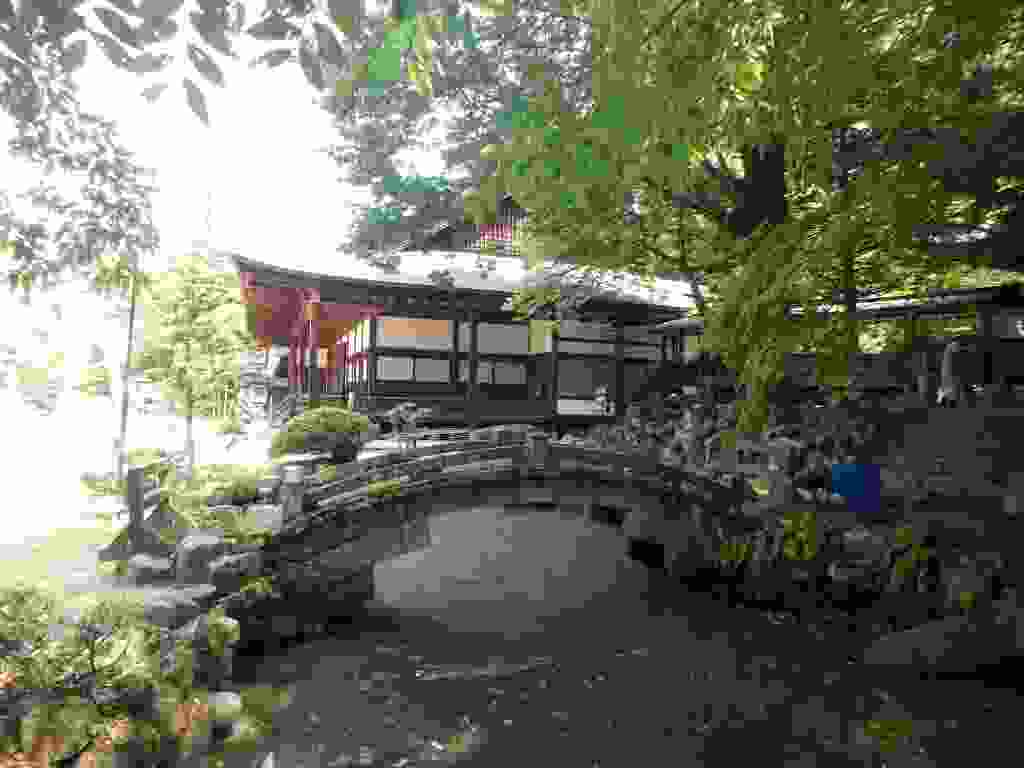
\includegraphics[width=\mywidth]{../wp-content/uploads/2015/08/P8076059-1024x768.jpg} \end{center}

 

 A coté de Takayama, un petit village de montagne reconstitué avec des maisons typiques au toit très pentu. 

 

\begin{center} 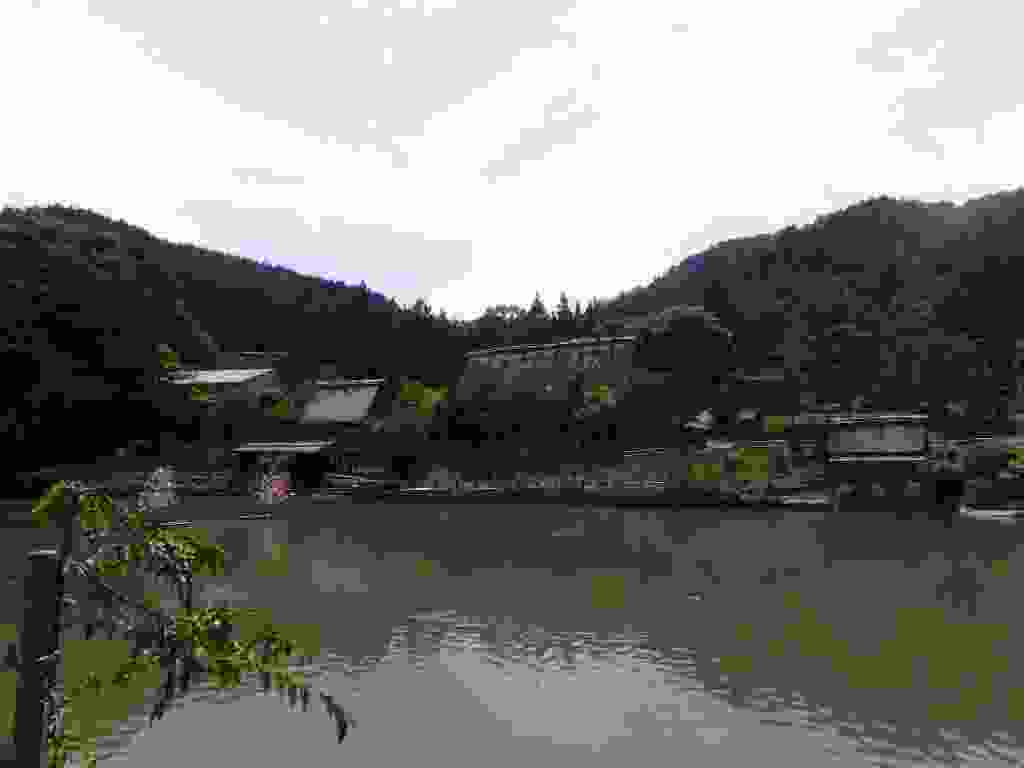
\includegraphics[width=\mywidth]{../wp-content/uploads/2015/08/P8076066-1024x768.jpg} \end{center}

 

 

\begin{center} 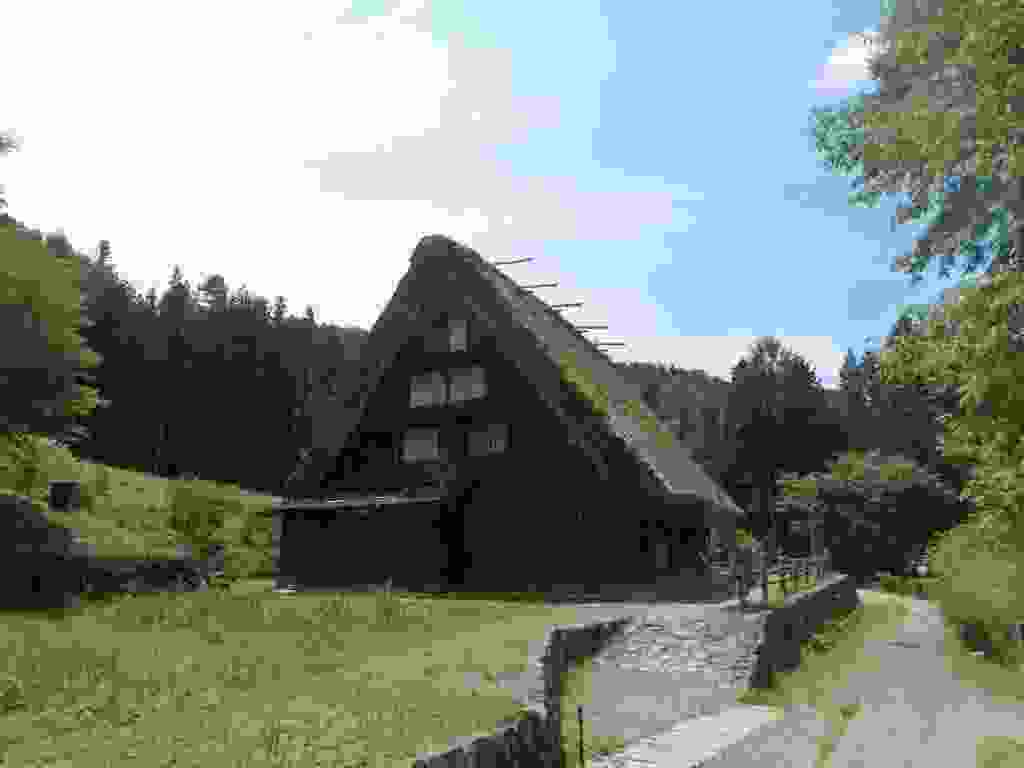
\includegraphics[width=\mywidth]{../wp-content/uploads/2015/08/P8076068-1024x768.jpg} \end{center}

 

 

\begin{center} 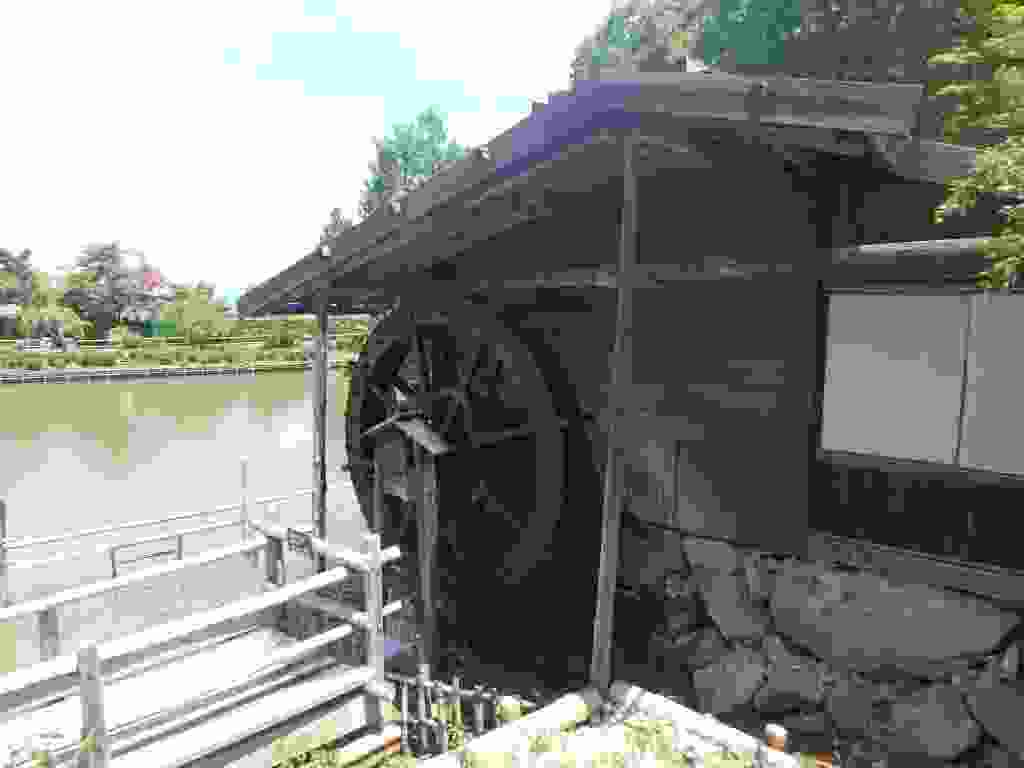
\includegraphics[width=\mywidth]{../wp-content/uploads/2015/08/P8076069-1024x768.jpg} \end{center}

 

 

\begin{center} 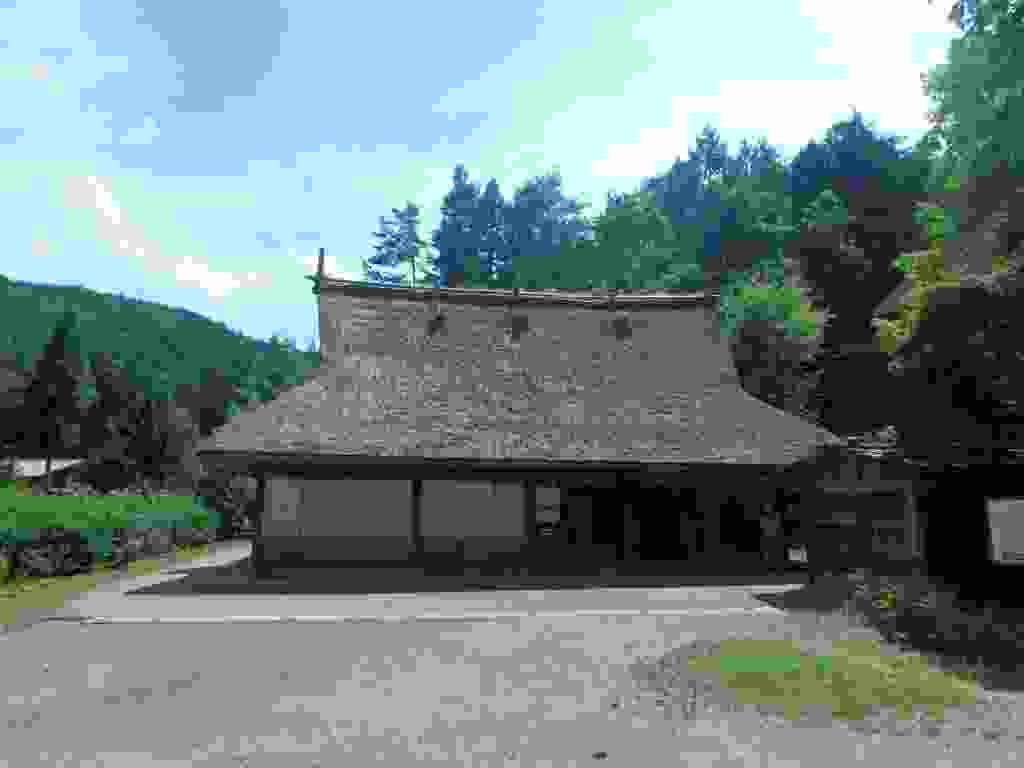
\includegraphics[width=\mywidth]{../wp-content/uploads/2015/08/P8076074-1024x768.jpg} \end{center}

 

 

\begin{center} 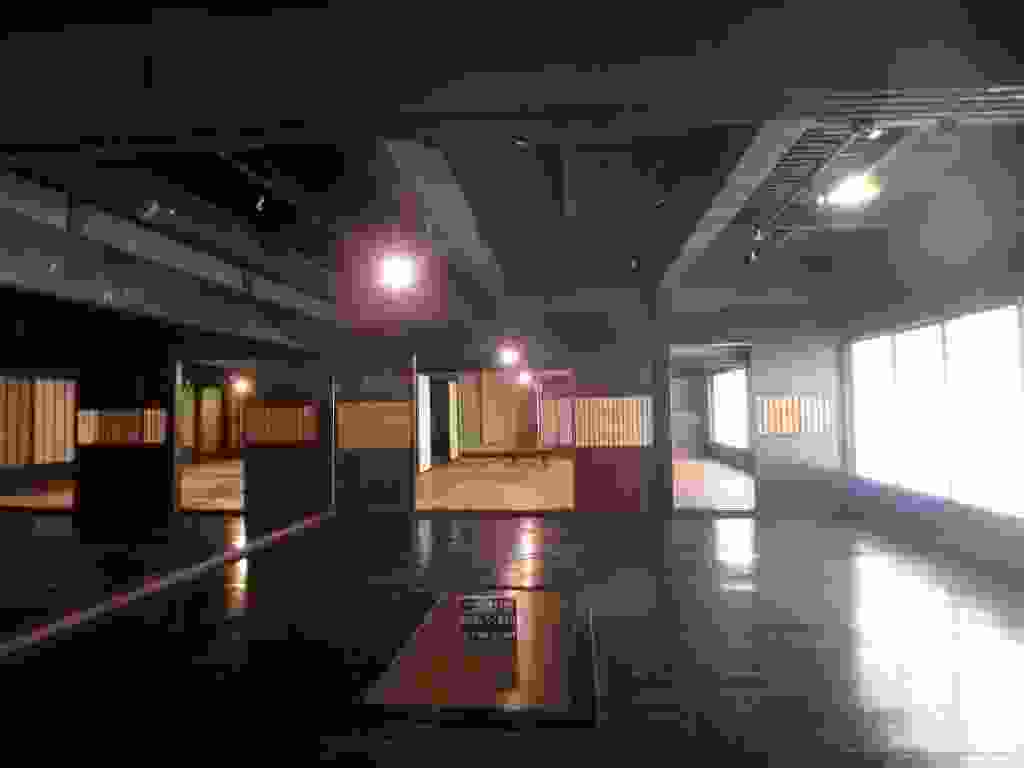
\includegraphics[width=\mywidth]{../wp-content/uploads/2015/08/P8076072-1024x768.jpg} \end{center}

 

 Je teste le boeuf de Hida très réputé au Japon. 

 

\begin{center} 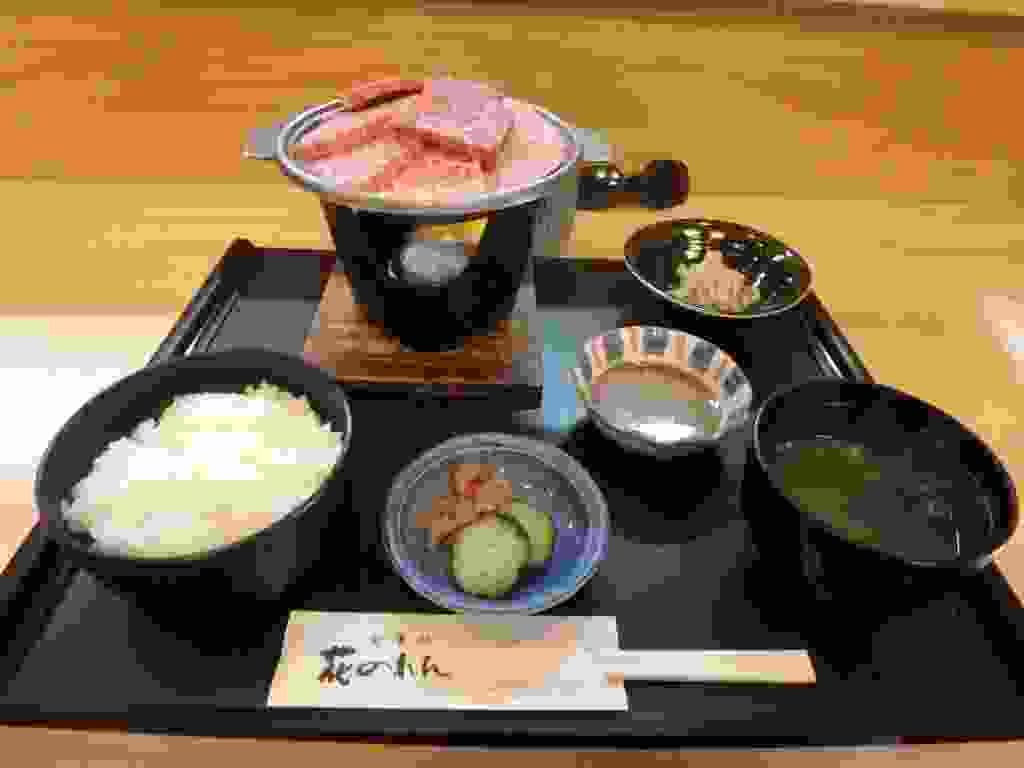
\includegraphics[width=\mywidth]{../wp-content/uploads/2015/08/P8076077-1024x768.jpg} \end{center}

 

 Je roule ensuite vers Shirakawago, village inscrit à l'Unesco avec une centaine de maisons traditionnelles comme les précédentes. Je m'aperçois que le col pour y accéder est fermé, ce qui m'oblige à un grand détour. Finalement je renonce à Shirakawago et je descends vers la petite ville de Gujō. 

 

\begin{center} 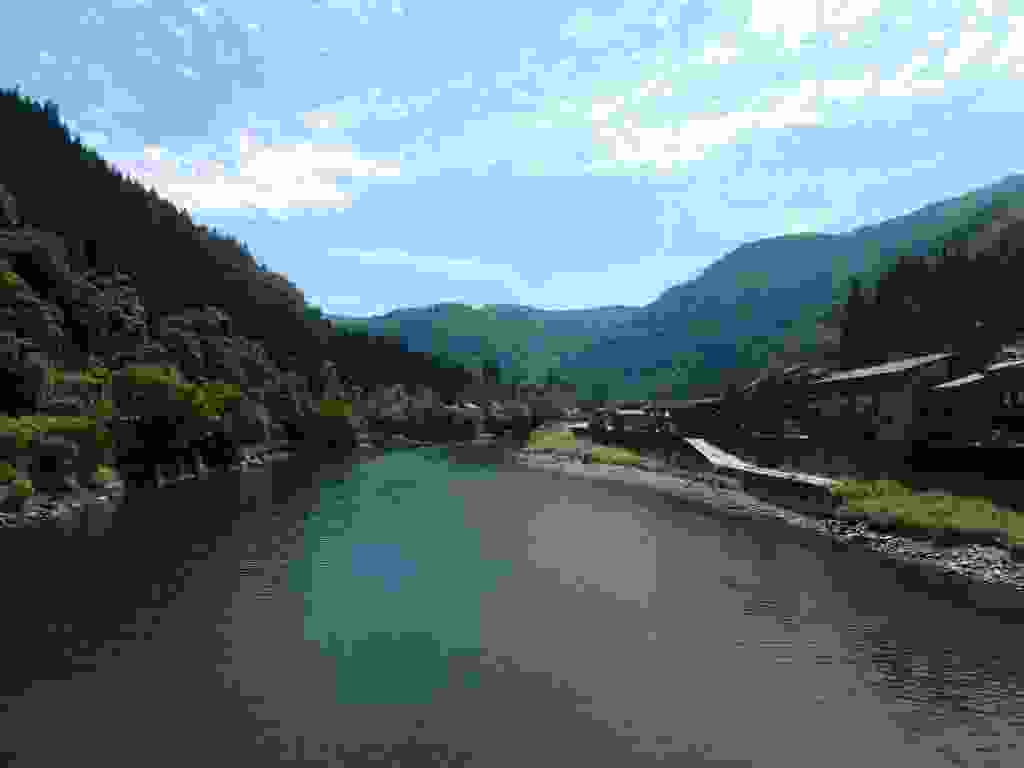
\includegraphics[width=\mywidth]{../wp-content/uploads/2015/08/P8086081-1024x768.jpg} \end{center}

 

 

\begin{center} 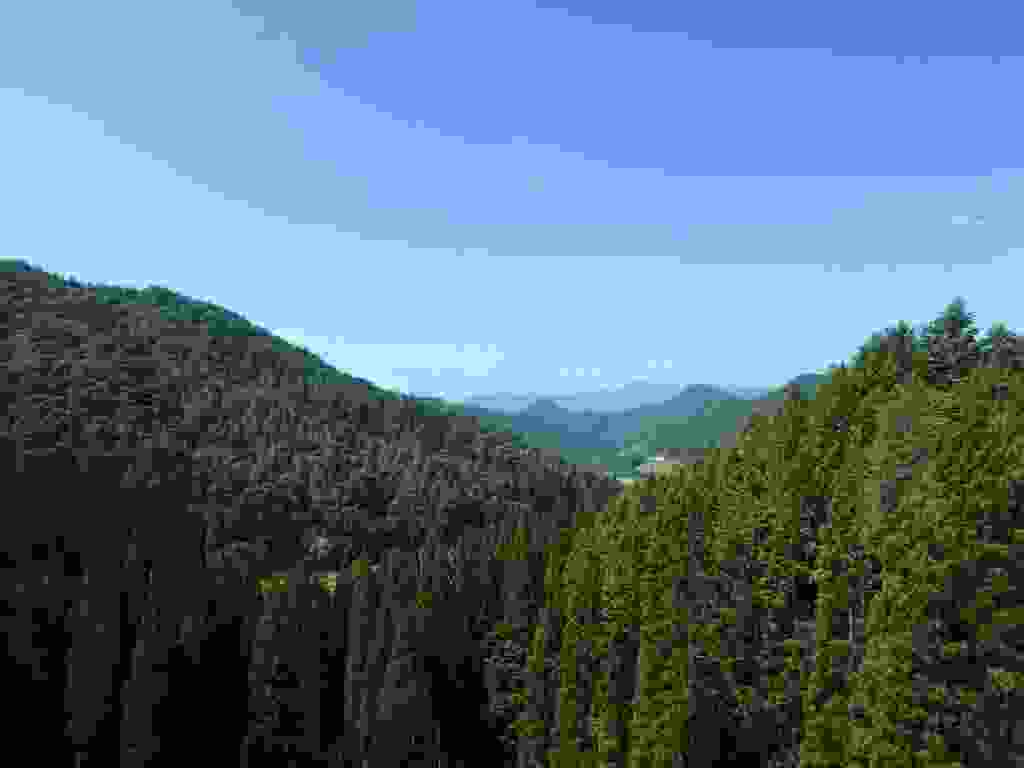
\includegraphics[width=\mywidth]{../wp-content/uploads/2015/08/P8086085-1024x768.jpg} \end{center}

 

 

\begin{center} 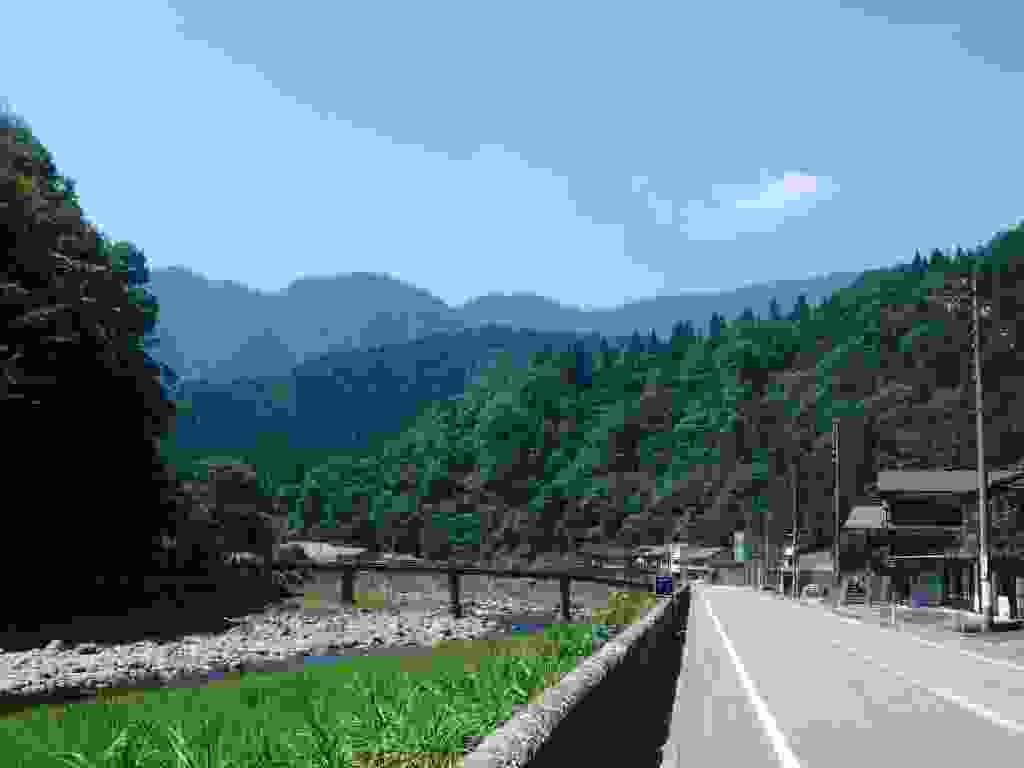
\includegraphics[width=\mywidth]{../wp-content/uploads/2015/08/P8096092-1024x768.jpg} \end{center}

 

 Chateau de Gujō perché sur une colline. 

 

\begin{center} 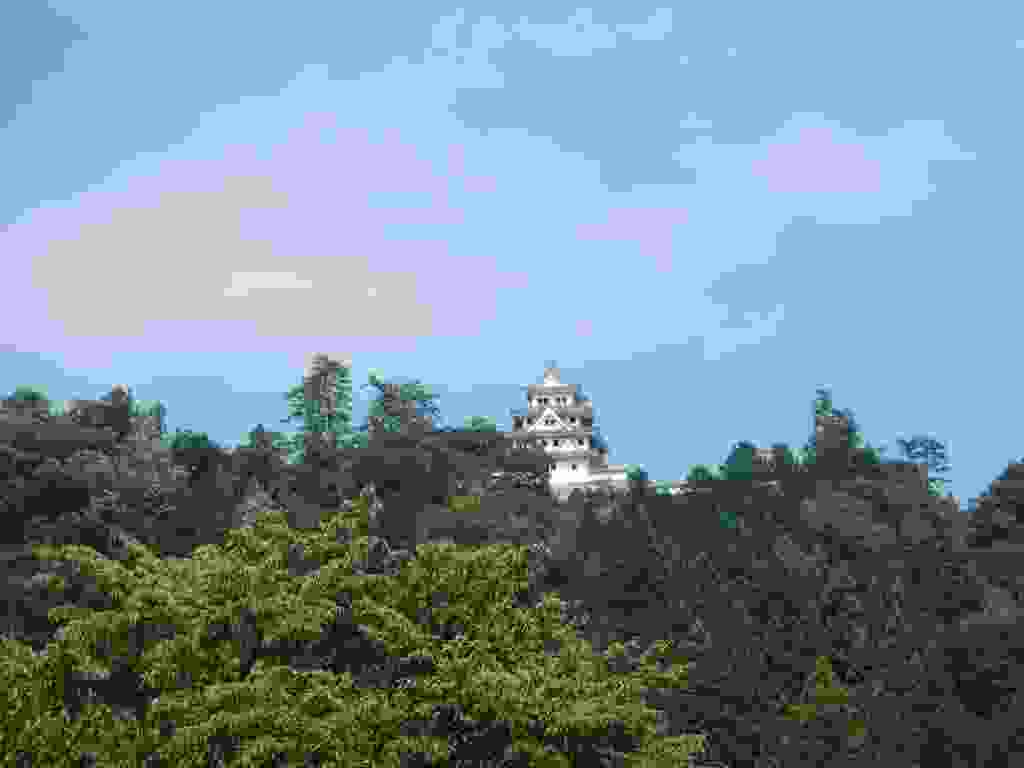
\includegraphics[width=\mywidth]{../wp-content/uploads/2015/08/P8096111-1024x768.jpg} \end{center}

 

 

\begin{center} 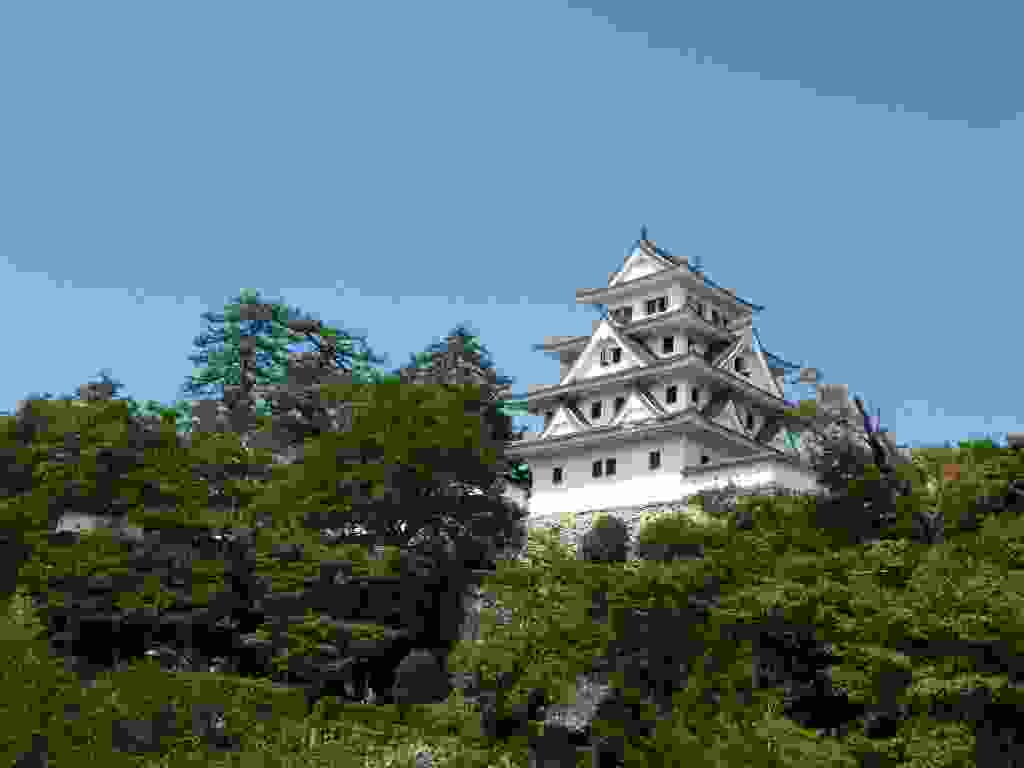
\includegraphics[width=\mywidth]{../wp-content/uploads/2015/08/P8096100-1024x768.jpg} \end{center}

 

 Belle rivière ou beaucoup de monde se baigne ou pêche. 

 

\begin{center} 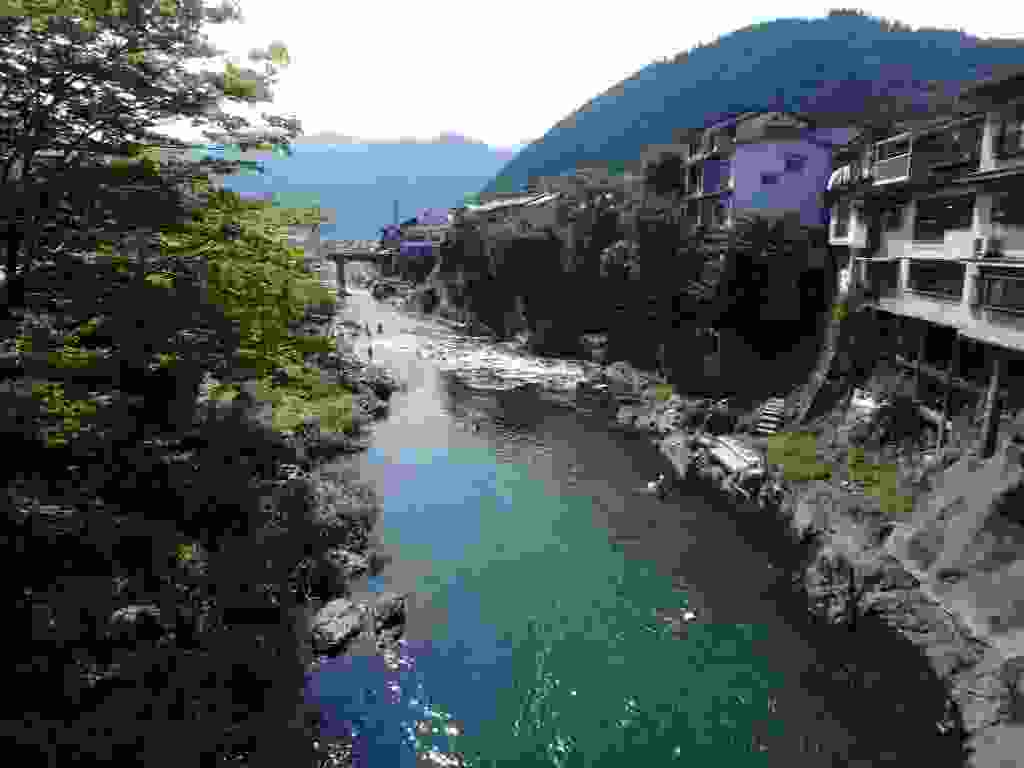
\includegraphics[width=\mywidth]{../wp-content/uploads/2015/08/P8096094-1024x768.jpg} \end{center}

 

 

\begin{center} 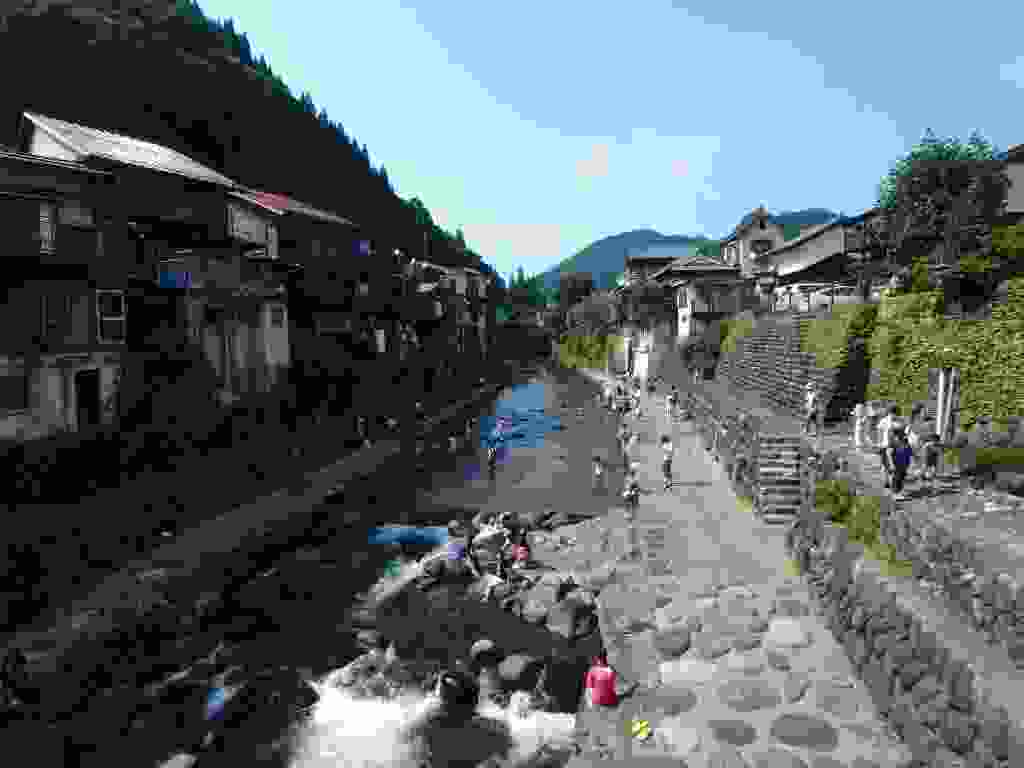
\includegraphics[width=\mywidth]{../wp-content/uploads/2015/08/P8096113-1024x768.jpg} \end{center}

 

 Plusieurs ruelles avec des canaux. 

 

\begin{center} 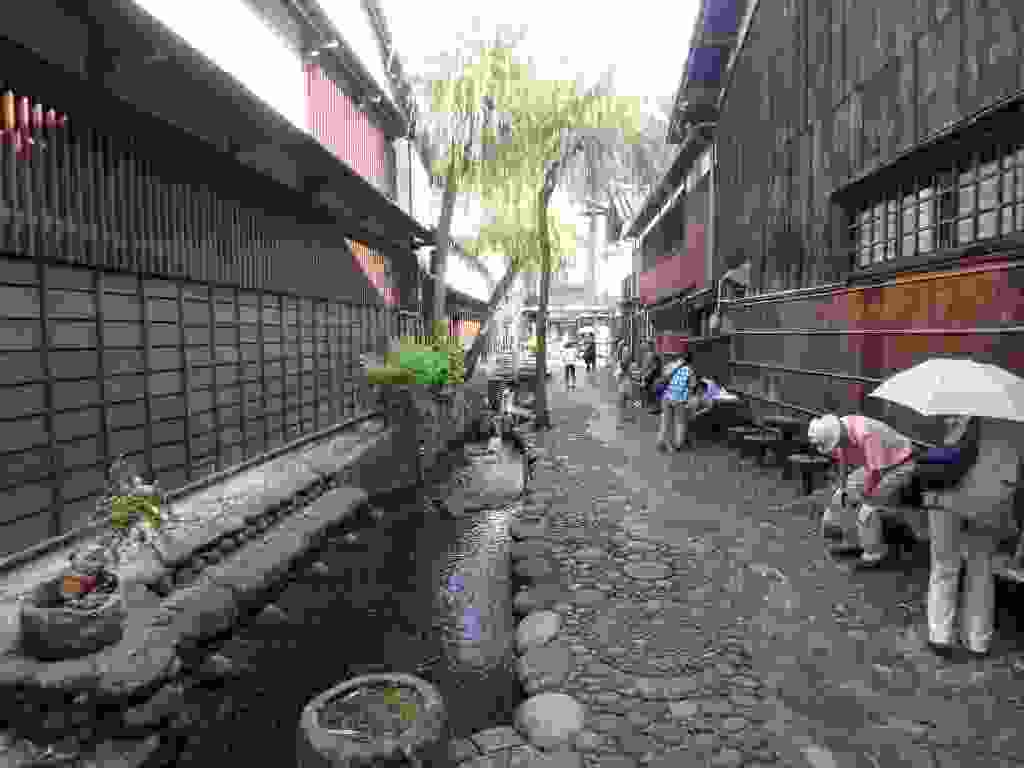
\includegraphics[width=\mywidth]{../wp-content/uploads/2015/08/P8096116-1024x768.jpg} \end{center}

 

 

\begin{center} 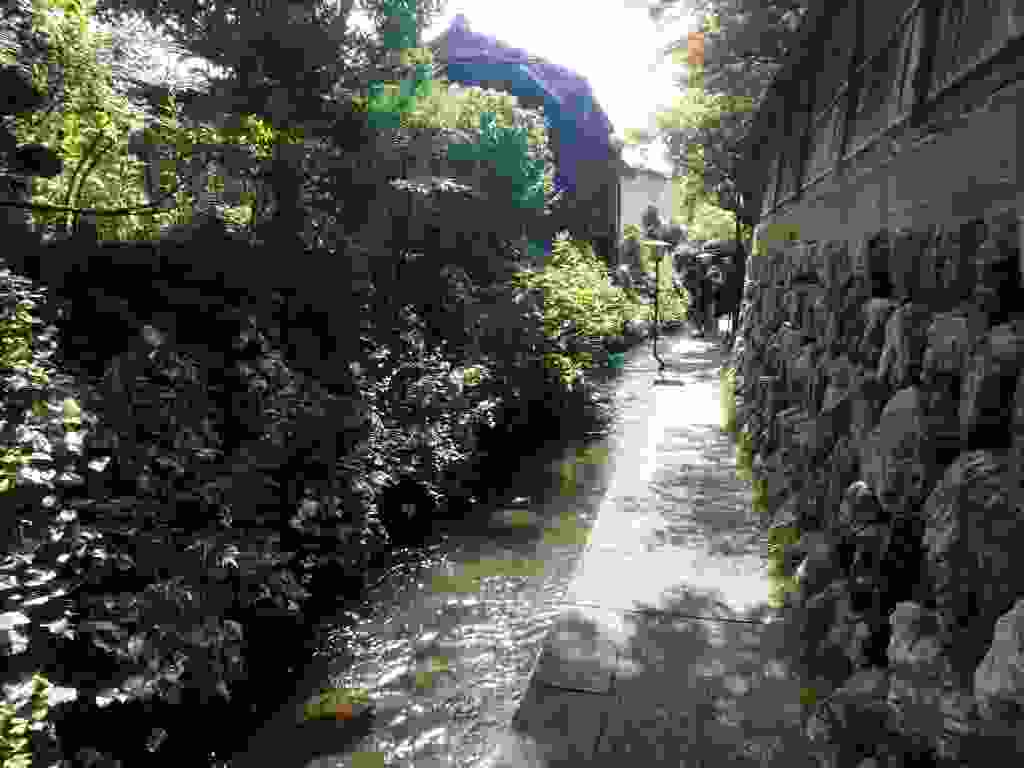
\includegraphics[width=\mywidth]{../wp-content/uploads/2015/08/P8096096-1024x768.jpg} \end{center}

 

 Source d'eau très pure au coeur de la ville. 

 

\begin{center} \includegraphics[width=\mywidth]{../wp-content/uploads/2015/08/P8096114-1024x768.jpg} \end{center}

 

 C'est de Gujō que sont originaires les reproductions de plats des restaurants japonais. On peut en acheter des centaines de différentes dans cette boutique. 

 

\begin{center} \includegraphics[width=\mywidth]{../wp-content/uploads/2015/08/P8096115-1024x768.jpg} \end{center}

 

 Tout l'été, un festival de danse a lieu dans une rue différente chaque soir. La plupart des gens dansent et beaucoup portent le kimono, belle ambiance. 

 

\begin{center} \includegraphics[width=\mywidth]{../wp-content/uploads/2015/08/P8096123-1024x768.jpg} \end{center}




 
 
